\documentclass[11pt,a4paper,twoside]{report}
\usepackage[portuguese]{babel}
\usepackage{graphicx}  		%% display images
\usepackage{float}			%% make graphics float in place
\usepackage{indentfirst}
\usepackage{hyphenat}
\usepackage{subcaption}		%% allows for subgigures
\usepackage{listings} 		%% for listing code
\usepackage[top=2.50cm, bottom=2.50cm,left=2.50cm, right=2.50cm]{geometry} % margens
\usepackage[colorlinks=true,linkcolor=black,urlcolor=black,bookmarksopen=true]{hyperref} %% Make hyperlinks in index
\usepackage{bookmark} 		% Bookmarks for pdf file
%\renewcommand{\baselinestretch}{1.2} 
\usepackage{fancyhdr} 		% creates fancy footers and headers
\pagestyle{fancy}
\lfoot{{\footnotesize Tecnologias de Informação}}
\rfoot{{\footnotesize ESTGA}}
\rhead{Projecto Temático em Desenvolvimento de Aplicações}
\lhead{}
%\author{}
%\date{}
\makeindex
\usepackage{tabularx}

\begin{document}
%\maketitle


\begin{titlepage}
	\centering
	\vfill
	
\includegraphics[width=7cm]{image/ESTGA} % also works with logo.pdf
	\vfill
	
	{\bfseries\Large
		Projeto temático em Desenvolvimento de Aplicações\\
		Relatório \\
		\vskip2cm
		%A. Uthor\\
	}    
	
	\vfill
	\textbf{Grupo 5}
	
	António Bento (97737)
	
	Diogo Matos (98017)
	
	Ivan Xavier (92441)
	
	Maykol Santos (74079)
	
	Ricardo Fernandes (49880)
	
	Simão Julião (98045)
	\vfill
\end{titlepage}



\pagenumbering{roman}
%\begin{small}
	\tableofcontents
%\end{small}

\pagenumbering{roman}
\listoffigures
\newpage\null\thispagestyle{empty}\newpage
\pagenumbering{arabic}





\chapter{Introdução}

No âmbito do Projeto Temático em Desenvolvimento de Aplicações o Grupo 5 propôs-se desenvolver uma aplicação de gestão de uma clínica dentária, utilizando os conhecimentos adquiridos nas unidades curriculares de Engenharia de Software e Sistemas de Base de Dados incluídas no plano curricular da licenciatura em Tecnologias de Informação, ministrada na Escola Superior de Tecnologia e Gestão de Águeda – Universidade de Aveiro.

Os requisitos a cumprir no final do projeto foram identificados e desenvolvidos no decorrer de cinco reuniões entre a equipa e o representante do cliente, onde foi debatido a ideia geral do sistema.

Nestas reuniões foram abordados diversos temas que definem o funcionamento do projeto e irão ser a estrutura deste relatório nos capítulos de levantamento e desenvolvimento de requisitos do projeto.

Inicialmente, foi discutida a ideia geral do projeto onde surgiu a ideia do \textit{software} para gestão de uma clínica, que mais tarde foi especializada para aplicações de medicina dentária.
Após escolhido o tema principal do projeto foi escolhida a linguagem de programação que define o rumo do projeto.
Esta originalmente estaria pré-definida por orientações dos Professores, sendo Java a língua escolhida por estar inserida no contexto académico do curso de Tecnologias de Informação, contudo foi concedida liberdade criativa ao grupo de escolher uma alternativa que satisfaça as condições de ser uma língua orientada a objetos.

Estando as formalidades iniciais completas, foram definidas as funcionalidades que o \textit{software} deve conter e o que seria útil mas não prioritário.
Dentro destas funcionalidades, foram levantados problemas naturais de restrições de acesso a funcionalidades ou a informações de doentes, estas têm de ser implementadas no código de forma a este estar em conformidade com requisitos legais.
Além destas, salientou-se a necessidade de manter a integridade da base de dados que foi ser implementada.

Dentro da parte mais técnica do pré desenvolvimento do projeto foi desenvolvido, durante várias reuniões com o orientador, os Diagramas de Atividades, os Diagramas de Classes e a Estrutura de Dados que juntos formam o esqueleto do projeto e o guia principal para orientar o desenvolvimento do código.
Dado que este projeto consiste numa ferramenta de gestão para uma clínica, o sistema de \textit{Login} é então um dos focos principais a desenvolver já que define a diferenciação de classes a ser implementadas e a forma como interagem entre si, assim como define a estrutura de como o interface irá ser desenvolvido.

Estes temas aqui referidos serão mais desenvolvidos no decorrer do relatório com capítulos inteiramente dedicados aos tópicos mais cruciais.

%Temas abordados: 
%
%\begin{itemize}
%	\item   Ideia geral do projeto 
%	\item   Restrições e Integridade 
%	\item   Funcionalidades a adicionar 
%	\item	Linguagem de desenvolvimento 
%	\item	Diagramas de casos de uso
%	\item	Funcionalidades definidas
%	\item	Diagramas de atividades 
%	\item	Diagramas de classes 
%	\item	Estrutura de dados 
%	\item   Sistema de login 
%	
%\end{itemize}
%\pagebreak
\section{Visão geral do sistema }

O projeto consiste na criação de \textit{software} para gestão de uma clínica dentária.
Este consiste numa interface desenvolvida para as necessidades dos diferentes cargos de funcionários da empresa ao mesmo tempo que é estabelecida uma comunicação com a base de dados, onde todos os dados serão guardados.
Com o objetivo de desenvolver a mesma, foram levantados requisitos e necessidades que mais tarde definiram funcionalidades e estruturas do sistema.

O sistema irá registar a informação necessária dos profissionais da clínica e dos utentes.
Vai também guardar a informação sobre consultas, possíveis exames e poderá imprimir receitas, relatórios de consulta e justificações.
As funcionalidades da aplicação estarão divididas por profissão, sendo que existirão diferentes tipos de permissões para cada tipo de utilizador.


\section{Cliente}

Este projeto consta com a presença de um cliente hipotético sendo este um representante de uma clínica de medicina dentaria.
Este tem o cargo de informar a equipa de desenvolvimento sobre os requisitos e funcionalidades necessárias a implementar no sistema, requisitos de segurança e de conformidade legal como proteção de dados sensíveis como também dos prazos de entrega e formalidades do mesmo.
Foi assim possível definir objetivos concretos e realistas inerentes ao projeto a serem desenvolvidos durante o decorrer deste projeto.

\section{Objetivos}

Tendo em conta que a clínica dentária tem a necessidade de gerir e controlar todos os seus clientes e profissionais, bem como todos os dados relacionados com os mesmos (consultas, exames, ficha de cliente, ficha de profissional, entre outros) existe a necessidade de armazenar e gerir os dados necessários para permitir o correto funcionamento da clínica dentária.
Considerando o que foi referido, é necessário criar uma aplicação capaz de responder aos requisitos previamente indicados, a equipa de desenvolvimento tem como objetivo fornecer coesão e estrutura para que seja possível desenvolver a aplicação em questão, de um modo eficaz e fluído.

O cliente pretende que o sistema apresente uma alternativa moderna e competente à solução anterior. Para que tal se realize, a solução apresentada pela equipa de desenvolvimento tem a obrigação de estar apta para suportar todas as funcionalidades indispensáveis à clínica. 

Com esta alteração de sistema existem benefícios não só de desempenho como de utilidade, no sentido em que as operações passam a ser instantâneas e é possível aceder à informação que é constantemente atualizada e validada, este é o mesmo conceito que possibilita a uniformidade de sistema (prevenção de falhas na integridade), permite uma validação e verificação ativa de dados aquando registados, permite desenvolvimento futuro, permite armazenamento de enormes quantidades de informação e retira todas as inconveniências de um sistema de registos tradicional.

%\begin{itemize}
%	\item     	Atualização de dados e verificação dos mesmos em tempo real. 
%	\item	  	Uniformidade superior de sistema e menor possibilidade/probabilidade de erros. 
%	\item		Autonomia de sistema em atualização de dados e gestão de clientes.
%	\item	    Sistema interativo a capaz de crescimento. 
%	\item 	    Capacidade de não depender de registos físicos. 
%\end{itemize}

\section{Desafios de Crescimento Profissional}

Por forma a desenvolver o nosso crescimento profissional fora das expectativas institucionalizadas e também de satisfazer conquistas pessoais, o grupo auto propôs-se ao desafio de usar a linguagem de programação Python em vez de Java como estava proposto na orientação da disciplina.

A linguagem Python tem vindo a crescer na sua adoção com o passar dos anos, tornando-se numa ferramenta versátil de programação a alto nível usada por várias instituições académicas e empresariais em diversas áreas, onde de momento se destacam os tópicos mais mediáticos como \textit{machine learning}, cibersegurança\cite{KukMilSpaGoc19} e aplicações científicas.
A sua abordagem orientada para algoritmos permite desenvolvimento rápido de projetos que são fundamentais para prototipagem\cite{Redondo_2015}, o esforço das comunidades dedicadas resultaram em bibliotecas extensas de alta qualidade que permitem criação de código eficiente, capaz de ser mais rápido e consumindo menos memória que Java em determinadas aplicações\cite{KukMilSpaGoc19}.

Publicações recentes mostram que Python está a evoluir corretamente no que toca a mitigação de vulnerabilidades e desenvolvimento de funcionalidades, que permitem melhor segurança em aplicações online.\cite{khwaja+murtaza+ahmed2020}.

Visto que Python não dispõe dos mesmos métodos de criação de interface que estão presentes num IDE de Java, como o JFrame, foi necessário escolher uma framework que tivesse compatibilidade  com Python e que satisfaça as necessidades modernas de funcionamento com \textit{desktop}, \textit{mobile} e sistemas \textit{embedded}.
Tendo isto em consideração, foi escolhido a Qt \textit{framework} que é de código livre e funciona com quaisquer sistemas operativos modernos. 
Com Qt \textit{framework} e o \textit{software} de desenvolvimento de interface, \textbf{Qt Designer}, é possível desenvolver uma interface que funcione e se adapte para vários dispositivos diferentes com tamanhos de ecrã e resolução muito diferentes. 
Esta aplicação e as suas bibliotecas são compatíveis e compiladas por compiladores standard de C++. garantindo assim a sua compatibilidade com projetos que usem compiladores específicos de C++, e do lado do utilizador, um produto final de execução rápida e leve em recursos computacionais\cite{Neto2017}.
A interação entre as interfaces geradas e as bibliotecas de Qt com Python é feita com recurso à biblioteca \textbf{PyQt}.




\chapter{Modelo de requisitos}

\section{Requisitos funcionais }

Os requisitos funcionais do sistema foram debatidos em grupo de forma a definir a sua prioridade de implementação.
Estes podem ser consultados na tabela seguinte:

\begin{tabularx}{\textwidth}{|l|X|c|}
	\hline
\textbf{Refª} 	& \textbf{Requisito funcional}   & \textbf{Prioridade}  \\
	\hline
RF.1 	& Guardar os dados dos utentes  & Alta  \\
	\hline
RF.2	& O sistema tem de registar profissionais  & Alta \\
	\hline
RF.3	& Tem de existir um método de autenticação de funcionários  & Alta \\
	\hline
RF.4	& Criação da ficha de cliente  & Alta  \\
	\hline
RF.5	& Criação do relatório médico  & Alta \\
	\hline
RF.6	& Registar o estado do paciente no relatório  & Alta \\
	\hline
RF.7	& Registar a prescrição do paciente no relatório  & Alta \\
	\hline
RF.8	& Consultar a ficha do utente  & Alta \\
	\hline
RF.9	& Consultar o relatório do utente  & Alta \\
	\hline
RF.10	& Aceder a relatórios de consultas anteriores  & Alta \\
	\hline
RF.11	& Alterar o relatório de utente  & Alta  \\
	\hline
RF.12	& Consultar prescrição médica  & Alta  \\
	\hline
RF.13	& Adição de exames ao relatório  & Alta  \\
	\hline
RF.14	& Administrador capaz de gerir e alterar todos os dados e configurações  & Alta \\
	\hline
RF.15	& Agendar consultas  & Alta \\
	\hline
RF.16	& Verificação de sobreposição de consultas  & Média \\
	\hline
RF.17	& Facultar justificação médica   & Baixa \\
	\hline
RF.18	& Possibilidade de suspender o processo de utente  & Baixa \\
	\hline
RF.19	& Editar ficha de utente  & Alta \\
	\hline
\end{tabularx}

\section{Restrições e requisitos não funcionais }

\subsection{Requisitos de interface e facilidade de uso}

\paragraph{}

Para garantir padrões de satisfação e facilidade de uso, foram tidos em conta os seguintes pontos:

\begin{tabularx}{\textwidth}{|c|X|p{0.19\textwidth}|}
	\hline
\textbf{Refª} 	& \textbf{Requisito de interface e usabilidade}  & \textbf{Req. funcionais relacionados}  \\
	\hline
RInt.1 	& O sistema deve ter uma interface simples e acessível   &  \\
	\hline
RInt.2	& As cores do sistema devem ter em conta daltonismo  &  \\
	\hline
RInt.3	& O tamanho dos objetos e das letras deve ser equilibrado   &  \\
	\hline
\end{tabularx}

\subsection{Requisitos de desempenho  }

\paragraph{}

A equipa de desenvolvimento teve em consideração o desempenho e performance do sistema, com isto, foram definidas algumas restrições com o objetivo de garantir usabilidade.

\begin{tabularx}{\textwidth}{|c|X|p{0.19\textwidth}|}
	\hline
	\textbf{Refª} 	& \textbf{Requisito de desempenho }  & \textbf{Req. funcionais relacionados}  \\
	\hline
	RDes.1 	& As trocas de informação com a base de dados não devem exceder os 5000 milissegundos    &  \\
	\hline
	RDes.2	& Existe a necessidade de armazenar valores introduzidos pelo utilizador aquando introduzidos   & RF.19 \\
	\hline
	RDes.3	& Sincronização do sistema com o calendário e fuso horário local    &  \\
	\hline
	RDes.4	& Uso de uma base de dados segura e capaz de registar todos os dados pretendidos      &  \\
	\hline
	RDes.5	& Introdução de imagens de exames       & RF.13  \\
	\hline
	RDes.6	& Atualização de dados em tempo real	& \\
	\hline
\end{tabularx}

\subsection{Requisitos de segurança e integridade dos dados}

\paragraph{}

Atendendo às necessidades de cibersegurança e estabilidade da base de dados, foram estipuladas as seguintes normas:

\begin{tabularx}{\textwidth}{|c|X|p{0.19\textwidth}|}
	\hline
	\textbf{Refª} 	& \textbf{Requisito de segurança, privacidade e integridade de dados }  & \textbf{Req. funcionais relacionados}  \\
	\hline
	RSeg.1  & A entrada no sistema deve ser autenticada     & RF.3  \\
	\hline
	RSeg.2 	& O utilizador só pode realizar operações que lhe são permitidas    & RF.3  \\
	\hline
	RSeg.3 	& Cada operação deve ficar registada     &  \\
	\hline
	RSeg.4 	& A base de dados deve manter os dados       & RF.1  \\
	\hline
	RSeg.5	& A base de dados deve assegurar a integridade dos dados    & RF.1   \\
	\hline
\end{tabularx}


\subsection{Requisitos de interface com sistemas externos e com ambientes de execução }

\paragraph{}

Foram estipulados os seguintes requisitos funcionais relacionados com a compatibilidade de sistemas operativos, linguagem de comunicação com base de dados e linguagem de ligação entre interface visual e base de dados:

\begin{tabularx}{\textwidth}{|c|X|p{0.19\textwidth}|}
	\hline
	\textbf{Refª} 	& \textbf{Requisito de interface e usabilidade }  & \textbf{Req. funcionais relacionados}  \\
	\hline
	RIntE.1   & O sistema pode ser executado em sistemas Windows e Linux      &   \\
	\hline
	RIntE.2  	& O sistema comunica com uma base de dados MySQL     & RF.1   \\
	\hline
	RIntE.3  	& O sistema vai ser interpretado e executado em Python      &  \\
	\hline
\end{tabularx}

\subsection{Normas e regulamentação específicas aplicáveis}

\paragraph{}

Foram tomadas em conta as seguintes normas regulamentais relacionadas com cibersegurança e rastreabilidade de dados:

\begin{tabularx}{\textwidth}{|c|X|p{0.19\textwidth}|}
	\hline
	\textbf{Refª} 	& \textbf{Requisito de interface e usabilidade }  & \textbf{Req. funcionais relacionados}  \\
	\hline
	RReg.1    & Os dados fornecidos devem ser mantidos para fins legais.      &   \\
	\hline
	RReg.2 	  & Os dados fornecidos pelos clientes devem ser atuais e autênticos.    &    \\
	\hline
	RReg.3    & As palavras-chave devem estar encriptadas.       &  \\
	\hline
\end{tabularx}


\subsection{Outros requisitos não funcionais }

\paragraph{}

Para além dos requisitos estipulados acima, foram ainda definidos requisitos adicionais que complementam a integridade do programa, tais como:

\begin{tabularx}{\textwidth}{|c|X|p{0.19\textwidth}|}
	\hline
	\textbf{Refª} 	& \textbf{Requisito de interface e usabilidade  }  & \textbf{Req. funcionais relacionados}  \\
	\hline
	RnF.1     & Manutenção de erros inesperados do sistema.       &   \\
	\hline
\end{tabularx}


\section{Requisitos de hardware }

\paragraph{}

Os requisitos de hardware aqui apresentados são baseados nos sistemas de desenvolvimento disponíveis aos membros do grupo sendo que são exclusivamente limitados pelos meio disponiveis existentes, sendo estes:

\begin{tabularx}{\textwidth}{|c|X|p{0.19\textwidth}|}
	\hline
	\textbf{Refª} 	& \textbf{Requisito de Hardware}  & \textbf{Req. funcionais relacionados}  \\
	\hline
	RH.1      & Necessidade de um computador por posto de trabalho, com uma distribuição dos dois sistemas operativos principais (Windows e distribuições de Linux)     &  RF.16  \\
	\hline
	RH.2     & Necessidade de cada posto de trabalho ter acesso à Internet para ligação com a base de dados.   &   \\
\hline
	RH.3     & Necessidade de cada aplicação ser utilizada por um profissional   &   \\
\hline
\end{tabularx}

\chapter{Modelo de Casos de utilização}

\section{Visão geral}

\begin{figure}[H]
	\centering
	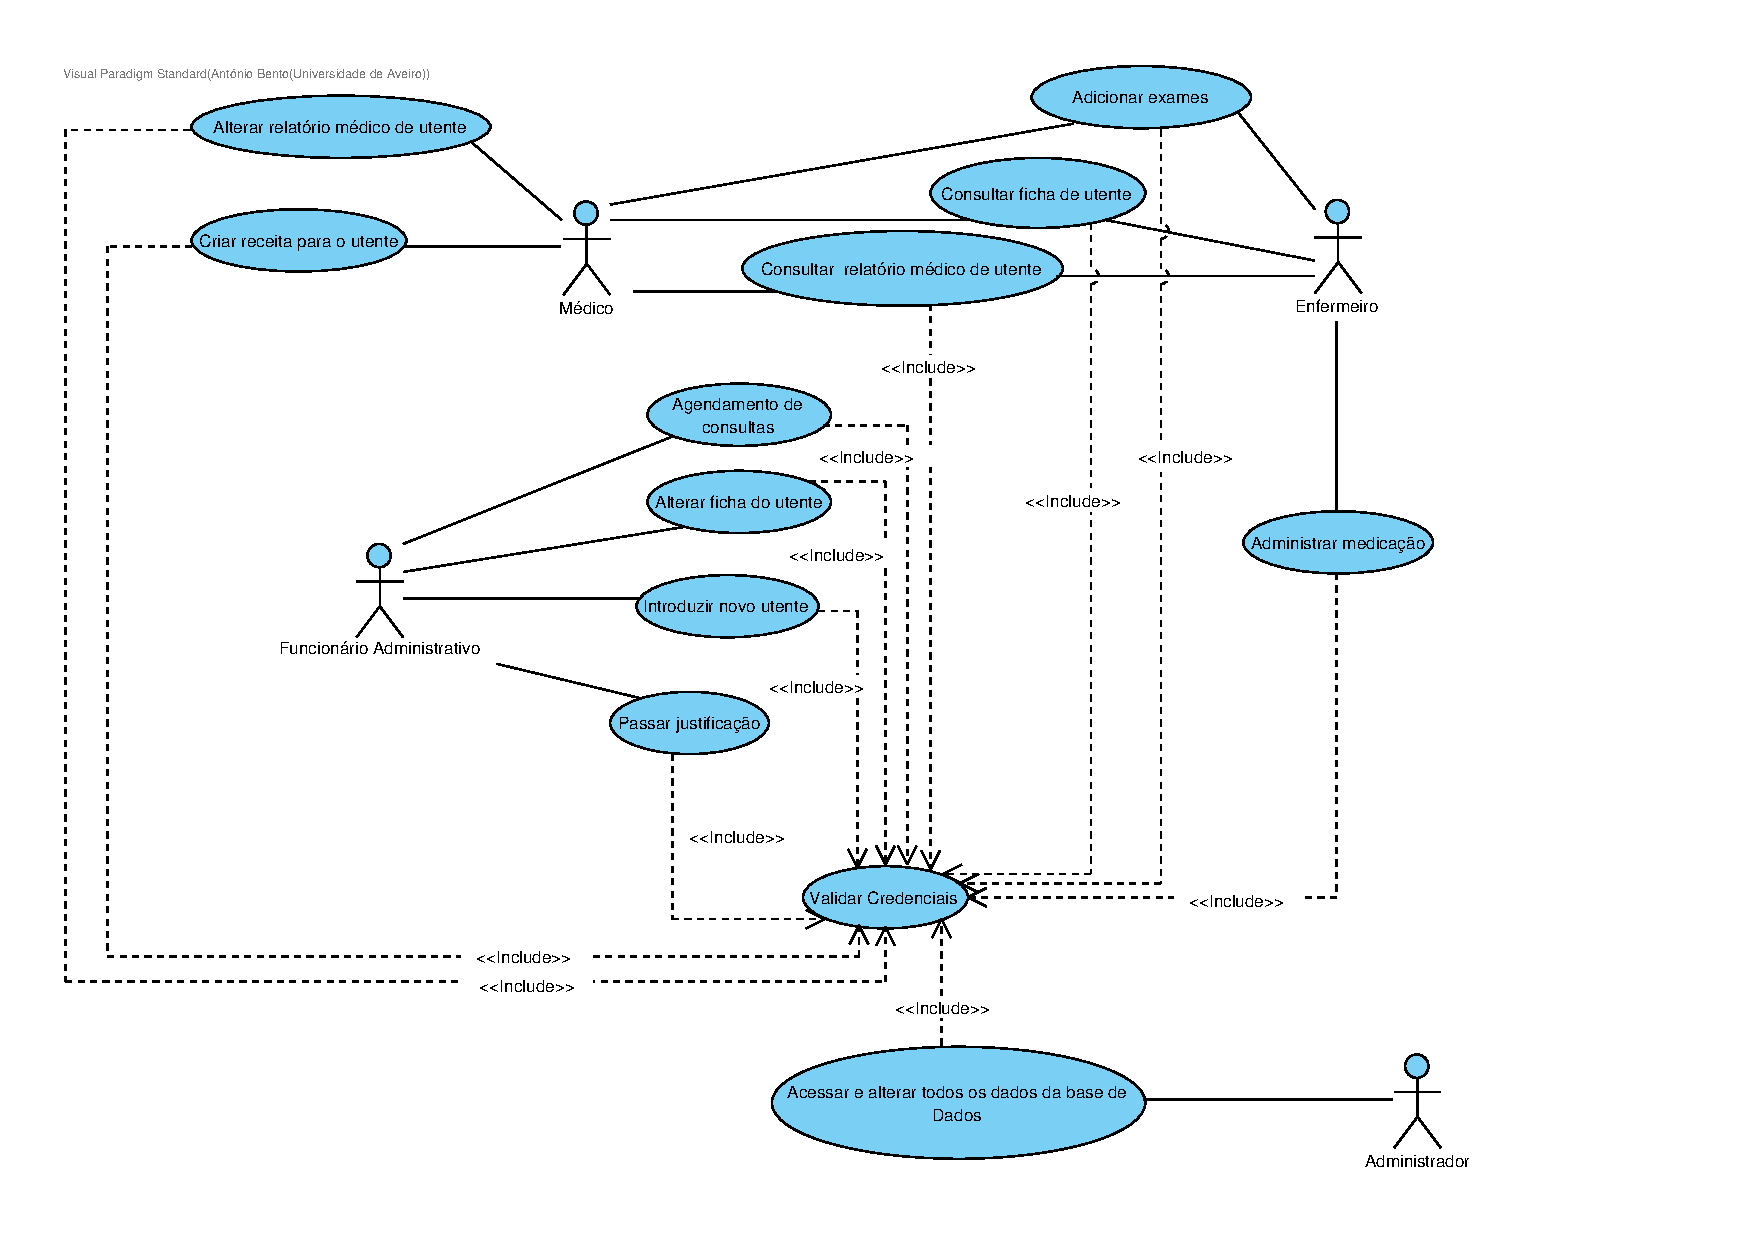
\includegraphics[width=0.95\linewidth]{image/Medico}
	\caption [Diagrama de Casos de Uso.] {Diagrama de Casos de Uso.}
	\label{fig:DiagramaCasoUso}
\end{figure}

Com a definição dos requisitos da clínica foi possível identificar funcionalidades e processos necessários para o correto funcionamento do sistema. Com isto, foi elaborado um diagrama de casos de uso que identifica e organiza as principais atividades que devem ser implementadas na aplicação.
É possível verificar, na figura \ref{fig:DiagramaCasoUso}, que cada ator está relacionado a um caso de uso, mas por particularidade, o sistema em questão, antecedendo à execução de qualquer atividade, o utilizador tem de ser validado com as respetivas credenciais. 

\section{Atores}

\paragraph{}
\begin{center}
	\begin{tabularx}{\textwidth}{|l|X|}
	\hline
	Ator & Descrição \\
	\hline
	Médico & Profissional de medicina dentária responsável por: \\
	&- Realizar consulta;  \\
	&- Consultar ficha de utente;   \\
	&- Consultar e alterar relatório médico; \\
	&- Adicionar exame. \\
	\hline
Enfermeiro & Profissional de saúde que auxilia o médico e executa certas tarefas individualmente, tais como: \\
	&- Consultar relatório medico e ficha de utente; \\
	&- Administrar medicação; \\
	&- Adicionar exames. \\
	\hline
Funcionário Administrativo & Funcionário da clínica responsável pelas tarefas administrativas, tais como: \\
	&- Introduzir novo utente; \\
	&- Alterar a ficha do utente; \\
	&- Conceder justificação médica. \\
	\hline
Utente  & 	Paciente que recorre à clínica para receber tratamento dentário \\
\hline
Administrador  & Responsável pelo bom funcionamento do sistema da clínica bem como gestão e verificação do mesmo. \\
\hline
\end{tabularx}
\end{center}

\section{Descrição dos casos de utilização }

\subsection{Validar Credenciais }

Um funcionário administrativo que pretende introduzir um novo utente, necessita de antes validar as suas credenciais introduzindo-as na interface do \textit{login} e verificar que estas são validadas pelo sistema de \textit{login}. 

\begin{center}
	\begin{tabularx}{\textwidth}{|lX|}
	\hline
	\textbf{Nome}: & \textbf{Validar Credenciais} \\ \hline
	Atores: & Administrador, Médico, Enfermeiro e Funcionário Administrativo \\ \hline
	Prioridade (1/3): & Alta \\ \hline
	Finalidade: & Validar o acesso ao sistema por parte de cada funcionário e isolar as suas permissões\\ \hline
	Requisitos & RF.5 \\
	Funcionais: & \\
	Pré-condições: & RF.18, RF.19, RF.20 e RF.21 \\
	Sumário: & Os funcionários da clínica quando abrem o software, são apresentados com uma interface com campos de texto para introduzir credenciais, que permitem identificar cada utilizador  \\
	\hline
\end{tabularx}

\begin{tabularx}{\textwidth}{|lX|}
	\hline
	\multicolumn{2}{|c|}{\textbf{Sequência típica dos eventos} }\\
\setlength{\tabcolsep}{12pt}
\textbf{Ações dos atores}  & \textbf{Respostas do sistema} \\
1. O profissional clica no executável & 1.1-     Apresenta uma interface para introduzir “Nome de utilizador” \\
2.     O profissional introduz o nome de utilizador & 1.2-    Apresenta uma interface para introduzir a “Password”  \\
3.    O profissional introduz a password & 4.1- Valida as credenciais na base de dados \\
4.    O funcionário confirma o pedido de acesso & 4.2- A base de dados confirma a validação \\
	& 4.3- A interface encaminha para a página associada ao profissional \\
	\hline
\multicolumn{2}{|c|}{\textbf{Sequências alternativas } }\\
\hline
\multicolumn{2}{|l|}{4.1.1- A base de dados invalida as credenciais   }\\
\multicolumn{2}{|l|}{4.2.1- O sistema devolve mensagem de erro    }\\
\multicolumn{2}{|l|}{4.3.1- O sistema mantém-se na página de acesso permitindo nova tentativa   }\\ \hline
\end{tabularx}

\end{center}

\begin{figure}[H]
	\centering
	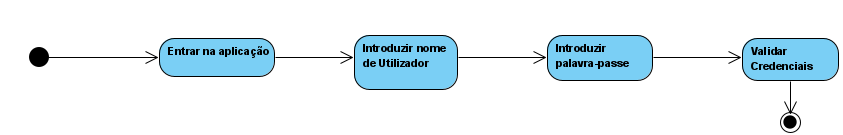
\includegraphics[width=0.7\linewidth]{image/Atividades/Validar Credenciais}
	\caption{Diagrama de atividades - Validar credenciais.}
	\label{fig:validarcredenciais}
\end{figure}



\subsection{Registar profissional }

O administrador procede ao preenchimento do formulário referente à criação de um novo profissional e atribui também as permissões conforme a profissão que o ator vá realizar. Após este preenchimento, o formulário é submetido e são guardadas as alterações no sistema. 

\begin{center}
	\begin{tabularx}{\textwidth}{|lX|}
		\hline
		\textbf{Nome}: & \textbf{Registar profissional} \\ \hline
		Atores: & Administrador \\ \hline
		Prioridade (1/3): & Alta \\ \hline
		Finalidade: & Registar funcionários no sistema e atribuir as devidas permissões \\ \hline
		Requisitos & RF.2, RF.3 e RF.4  \\
		Funcionais: & \\
		Pré-condições: & RF.18, RF.19, RF.20 e RF.21  \\
		Sumário: & O Administrador digita as credenciais no sistema, o sistema após a validação e seleciona a opção de criar um utilizador, é confrontado com um formulário onde pode associar profissões diferentes a cada utilizador.\\
		\hline
	\end{tabularx}
	
	\begin{tabularx}{\textwidth}{|XX|}
		\hline
		\multicolumn{2}{|c|}{\textbf{Sequência típica dos eventos} }\\
		\textbf{Ações dos atores}  & \textbf{Respostas do sistema} \\
		1. Introduz as credenciais no sistema  & 1.1-      Apresenta a opção de “Criar um funcionário”  \\
		2. O administrador preenche o formulário e associa a profissão a cada utilizador  & 1.2-  Apresenta um formulário para preencher sobre o funcionário   \\
		3.  O administrador submete o formulário  & 3.1- A estrutura de dados do formulário é validada  \\
		4.  O administrador clica no botão de saída  & 3.2- O sistema guarda os dados e credenciais na base de dados  \\
		& 3.3- O sistema atribui as devidas permissões a cada conta de utilizador  \\
		& 3.4- O sistema confirma operação \\
		& 3.5- O sistema mostra o botão de saída \\
		
		\hline
		\multicolumn{2}{|c|}{\textbf{Sequências alternativas } }\\
		\hline
		\multicolumn{2}{|l|}{1.1.1- Nega acesso e regista na base de dados o erro    }\\
		\multicolumn{2}{|l|}{3.1.1- Caso exista algum dado inválido, realça o mesmo e pede para voltar a introduzir     }\\
		\multicolumn{2}{|l|}{3.2.1- A comunicação com a base de dados não é possível  }\\ 
		\multicolumn{2}{|l|}{3.4.1- O sistema falha no registo do profissional   }\\ \hline
	\end{tabularx}
	
\end{center}

\begin{figure}[H]
	\centering
	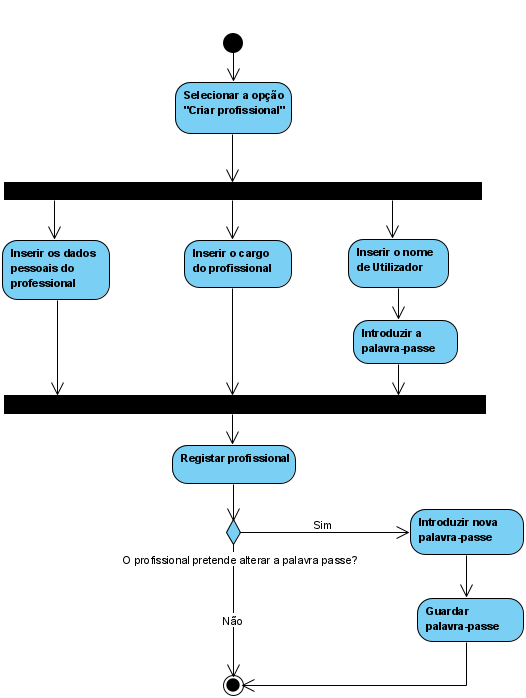
\includegraphics[width=0.6\linewidth]{image/Atividades/Registar Profissional}
	\caption{Diagrama de atividades - Registar profissional.}
	\label{fig:registarpessoal}
\end{figure}


\subsection{Introduzir novo utente}

Entra um utente que nunca tinha estado na clínica anteriormente. Este utente tem de ser adicionado à base de dados do sistema, ao criar uma ficha para o mesmo. O funcionário administrativo é o responsável por essa adição, pedindo um conjunto de dados ao utente para preencher o formulário. Após isto, o formulário é submetido e guardado no sistema.

\begin{center}
	\begin{tabularx}{\textwidth}{|lX|}
		\hline
		\textbf{Nome}: & \textbf{Introduzir novo utente} \\ \hline
		Atores: & Funcionário Administrativo  \\ \hline
		Prioridade (1/3): & Alta \\ \hline
		Finalidade: & Introduzir novo Utente na Clínica  \\ \hline
		Requisitos & RF.5, RF.6, RF.10   \\
		Funcionais: & \\
		Pré-condições: & O Funcionário Administrativo deverá ter credenciais para entrar no sistema    \\
		Sumário: & O funcionário deverá digitar as credenciais no sistema, para depois poder registar os dados o Utente no sistema e cria a ficha do Utente. Quando completo, o Utente fica registado no Sistema. \\
		\hline
	\end{tabularx}
	
	\begin{tabularx}{\textwidth}{|XX|}
		\hline
		\multicolumn{2}{|c|}{\textbf{Sequência típica dos eventos} }\\
		\textbf{Ações dos atores}  & \textbf{Respostas do sistema} \\
		1.     O funcionário regista os dados do Utente e cria a ficha do Utente   & 1.1-       O sistema guarda esses dados na base de dados   \\
		2.     Atribuir ao utente um médico   & 2.1-    O sistema guarda essa atribuição    \\
		3.      Agendar a primeira consulta   & 3.1-O sistema marca na agenda do médico essa consulta   \\
		&3.2 - O sistema regista o Utente com o sucesso  \\

		
		\hline
		\multicolumn{2}{|c|}{\textbf{Sequências alternativas } }\\
		\hline
		& \\
		 \hline
	\end{tabularx}
	
\end{center}

\begin{figure}[H]
	\centering
	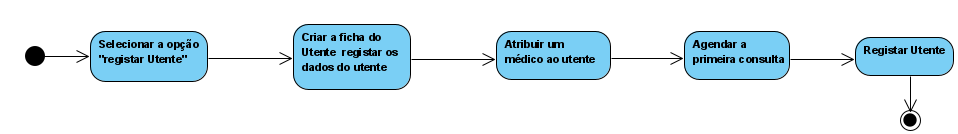
\includegraphics[width=0.7\linewidth]{image/Atividades/Introduzir novo utente}
	\caption{Diagrama de atividades - Introduzir novo utente.}
	\label{fig:introduzirnovoutente}
\end{figure}

\subsection{Alterar ficha do utente}

Um utente com ficha na clínica dirige-se à mesma com o intuito de marcar uma consulta mas, após uma verificação dos dados, repara que a sua morada não está atualizada e precisa de o fazer. Para isso, o funcionário administrativo acede à ficha do utente e procede então à alteração dos dados na ficha e guarda-as no sistema.  

\begin{center}
	\begin{tabularx}{\textwidth}{|lX|}
		\hline
		\textbf{Nome}: & \textbf{Alterar ficha do utente } \\ \hline
		Atores: & Funcionário Administrativo  \\ \hline
		Prioridade (1/3): & Alta \\ \hline
		Finalidade: & Alterar e atualizar a ficha do utente com novos dados   \\ \hline
		Requisitos & RF.5, RF.6    \\
		Funcionais: & \\
		Pré-condições: & O Funcionário Administrativo deverá ter credenciais para entrar no sistema    \\
		Sumário: & O funcionário deverá digitar as credenciais no sistema, para alterar os dados do Utente no sistema. Quando completo, o Utente fica com os seus dados atualizados na sua ficha de Utente. \\
		\hline
	\end{tabularx}
	
	\begin{tabularx}{\textwidth}{|XX|}
		\hline
		\multicolumn{2}{|c|}{\textbf{Sequência típica dos eventos} }\\
		\textbf{Ações dos atores}  & \textbf{Respostas do sistema} \\
		1.     O funcionário abre a ficha do utente    & 1.1-    O sistema disponibiliza a ficha \\
		2.     O funcionário modifica os dados do Utente    &   2.1-    O sistema guarda esses dados na base de dados  \\
		&  2.2 -     O sistema altera os dados com sucesso   \\
		&   \\
		\hline
		\multicolumn{2}{|c|}{\textbf{Sequências alternativas } }\\
		\hline
		& \\
		\hline
	\end{tabularx}
	
\end{center}

\begin{figure}[H]
	\centering
	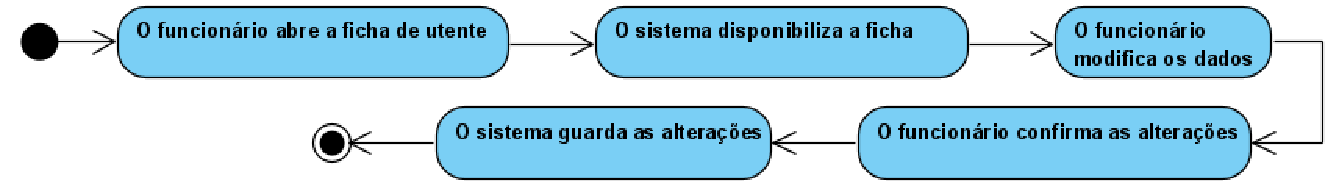
\includegraphics[width=0.7\linewidth]{image/Atividades/AlterarFichaUtente}
	\caption{Diagrama de atividades -   Alterar ficha do utente .}
	\label{fig:alterarfichautente}
\end{figure}


\subsection{Agendamento de consultas }

Um utente dirige-se à clínica com o intuito de marcar uma consulta. Este pede então ao funcionário administrativo, que irá abrir a agenda do médico de forma a verificar a disponibilidade, depois apresenta as opções ao utente que deve escolher a mais conveniente. Após a escolha, o funcionário de balcão confirma o agendamento da consulta em sistema e informa o seu correto agendamento. 

\begin{center}
	\begin{tabularx}{\textwidth}{|lX|}
		\hline
		\textbf{Nome}: & \textbf{Agendamento de consultas } \\ \hline
		Atores: & Funcionário Administrativo   \\ \hline
		Prioridade (1/3): & Alta \\ \hline
		Finalidade: & Agendar uma consulta para o utente    \\ \hline
		Requisitos & RF.5, RF.23    \\
		Funcionais: & \\
		Pré-condições: & O Funcionário Administrativo deverá ter credenciais para entrar no sistema    \\
		Sumário: & O funcionário deverá digitar as credenciais no sistema, para efetuar o agendamento da consulta na agenda do médico correspondente. Quando completo, o Utente fica com a próxima consulta marcada.  \\
		\hline
	\end{tabularx}
	
	\begin{tabularx}{\textwidth}{|XX|}
		\hline
		\multicolumn{2}{|c|}{\textbf{Sequência típica dos eventos} }\\
		\textbf{Ações dos atores}  & \textbf{Respostas do sistema} \\
		1.      O funcionário abre a agenda do médico     & 1.1-  O sistema disponibiliza a agenda  \\
		2.       O funcionário marca a consulta na agenda do médico     & 2.1-   O sistema verifica se o médico está disponível para essa consulta   \\
		& 2.2- O sistema marca a consulta com sucesso     \\
		\hline
		\multicolumn{2}{|c|}{\textbf{Sequências alternativas } }\\
		\hline
		\multicolumn{2}{|l|}{ O sistema poderá recusar a marcação da consulta devido a indisponibilidade do médico }\\
		\hline
	\end{tabularx}
	
\end{center}

\begin{figure}[H]
	\centering
	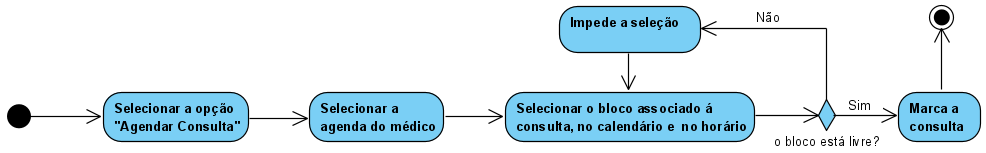
\includegraphics[width=0.7\linewidth]{image/Atividades/Agendamento de consultas}
	\caption {Diagrama de atividades - Agendamento de consultas.}
	\label{fig:agendamentoconsultas}
\end{figure}


\subsection{Passar justificação}

Após realizada uma consulta, um utente que esteja a faltar a um compromisso e que necessite de uma justificação, deve dirigir-se ao funcionário administrativo para a pedir. O funcionário preenche então o formulário da justificação e de seguida imprime a mesma, entregando-a ao utente. 

\begin{center}
	\begin{tabularx}{\textwidth}{|lX|}
		\hline
		\textbf{Nome}: & \textbf{Passar justificação } \\ \hline
		Atores: & Funcionário Administrativo   \\ \hline
		Prioridade (1/3): & Alta \\ \hline
		Finalidade: & Facultar justificação ao utente no caso de estar a faltar a algum compromisso como trabalho ou escola     \\ \hline
		Requisitos & RF.5, RF.24   \\
		Funcionais: & \\
		Pré-condições: & O Funcionário Administrativo deverá ter credenciais para entrar no sistema    \\
		Sumário: & O funcionário deverá digitar as credenciais no sistema, para depois preencher o formulário da justificação. Quando concluído, o funcionário imprime a justificação e entrega ao utente.   \\
		\hline
	\end{tabularx}
	
	\begin{tabularx}{\textwidth}{|XX|}
		\hline
		\multicolumn{2}{|c|}{\textbf{Sequência típica dos eventos} }\\
		\textbf{Ações dos atores}  & \textbf{Respostas do sistema} \\
		1.      O funcionário abre o formulário da justificação     & 1.1- O sistema disponibiliza o formulário  \\
		2.          O funcionário preenche os campos com os dados do utente      & 2.1- O sistema verifica que todos os campos estão preenchidos     \\
	    3. O funcionário imprime a justificação  & \\
	    4.  É entregue a justificação ao utente & \\
		\hline
		\multicolumn{2}{|c|}{\textbf{Sequências alternativas } }\\
		\hline
		\multicolumn{2}{|l|}{  }\\
		\hline
	\end{tabularx}
	
\end{center}

\begin{figure}[H]
	\centering
	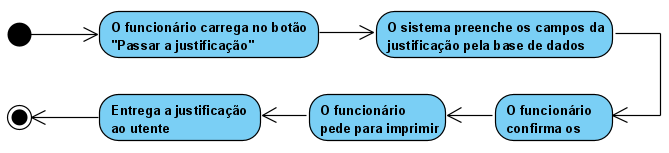
\includegraphics[width=0.7\linewidth]{image/Atividades/Justificação}
	\caption {Diagrama de atividades - Passar justificação.}
	\label{fig:passarjustificacao}
\end{figure}


\subsection{Criar receita para o utente }

Durante uma consulta, um médico repara numa infeção presente na boca do utente que necessita de tratamento antibiótico. O médico seleciona então a opção de criar uma receita para o utente, preenche os campos do formulário com as devidas informações. E depois o  funcionário Administrativo procede à sua impressão e entrega-a ao paciente no fim da consulta. 


\begin{center}
	\begin{tabularx}{\textwidth}{|lX|}
		\hline
		\textbf{Nome}: & \textbf{Criar receita para o utente } \\ \hline
		Atores: & Médico, Funcionário Administrativo   \\ \hline
		Prioridade (1/3): & Alta \\ \hline
		Finalidade: & Passar receita referente a algum medicamento ao utente   \\ \hline
		Requisitos & RF.3, RF.7    \\
		Funcionais: & \\
		Pré-condições: & O médico deverá ter credenciais para entrar no sistema   \\
		Sumário: & O médico deverá digitar as credenciais no sistema, para selecionar e preencher o formulário das receitas. Quando finalizado, o médico imprime a recita e entrega ao utente.  \\
		\hline
	\end{tabularx}
	
	\begin{tabularx}{\textwidth}{|XX|}
		\hline
		\multicolumn{2}{|c|}{\textbf{Sequência típica dos eventos} }\\
		\textbf{Ações dos atores}  & \textbf{Respostas do sistema} \\
		1.     O médico seleciona o formulário das receitas   & 1.1- O sistema apresenta o formulário   \\
		2.   O médico preenche com os dados necessários    & 2.1- O sistema verifica que todos os campos estão preenchidos    \\
		3.   O funcionário Administrativo imprime a receita    & 3.1- O sistema valida a receita e imprime  \\
	
		\hline
		\multicolumn{2}{|c|}{\textbf{Sequências alternativas } }\\
		\hline
		\multicolumn{2}{|l|}{  }\\
		\hline
	\end{tabularx}
	
\end{center}

\begin{figure}[H]
	\centering
	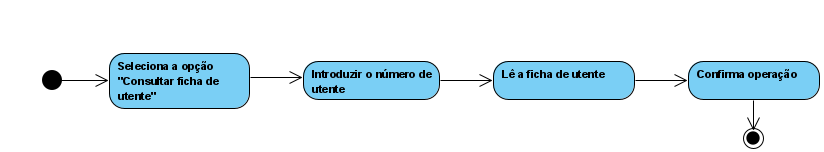
\includegraphics[width=0.7\linewidth]{image/Atividades/Criar receita}
	\caption{Diagrama de atividades - Criar receita para utente.}
	\label{fig:criarreceita}
\end{figure}


\subsection{Alterar relatório médico do utente }

Aquando a realização de uma consulta, é da responsabilidade do médico registar no sistema o resultado da mesma incluindo todos os detalhes necessários para que mais tarde seja possível verificar essa informação. 

\begin{center}
	\begin{tabularx}{\textwidth}{|lX|}
		\hline
		\textbf{Nome}: & \textbf{Alterar relatório médico do utente} \\ \hline
		Atores: & Médico   \\ \hline
		Prioridade (1/3): & Alta \\ \hline
		Finalidade: & Atualizar o relatório do utente    \\ \hline
		Requisitos & RF.3, RF.5, RF.11     \\
		Funcionais: & \\
		Pré-condições: &  O médico deverá ter credenciais para aceder ao sistema   \\
		Sumário: & O médico deverá digitar as credenciais no sistema, para selecionar o utente e poder alterar o relatório médico. Quando terminado, o relatório fica atualizado.  \\
		\hline
	\end{tabularx}
	
	\begin{tabularx}{\textwidth}{|XX|}
		\hline
		\multicolumn{2}{|c|}{\textbf{Sequência típica dos eventos} }\\
		\textbf{Ações dos atores}  & \textbf{Respostas do sistema} \\
		1.     O médico pesquisa o utente em questão    &   1.1-  O sistema apresenta a lista de utentes \\
		2.      O médico abre o relatório      & 2.1- O sistema apresenta a informação referente ao utente selecionado   \\
		3.      O médico altera o relatório conforme necessário     & 3.1-     O sistema guarda as alterações feitas no relatório   \\
		 4. O médico fecha o relatório  & \\
		
		\hline
		\multicolumn{2}{|c|}{\textbf{Sequências alternativas } }\\
		\hline
		\multicolumn{2}{|l|}{  }\\
		\hline
	\end{tabularx}
	
\end{center}

\begin{figure}[H]
	\centering
	\includegraphics[width=0.7\linewidth]{image/Atividades/AlterarRelatório}
	\caption{Diagrama de atividades - Alterar relatório médico do utente.}
	\label{fig:alterarrelatoriomedico}
\end{figure}


\subsection{Consultar relatório médico do utente }

Um cliente chega à consulta com o médico. O médico necessita então de rever o relatório médico do utente, para ter o ponto de situação sobre a consulta que vai realizar.

\begin{center}
	\begin{tabularx}{\textwidth}{|lX|}
		\hline
		\textbf{Nome}: & \textbf{Consultar relatório médico do utente } \\ \hline
		Atores: & Enfermeiro e médico    \\ \hline
		Prioridade (1/3): & Alta  \\ \hline
		Finalidade: & Consultar informação presente no relatório médico do paciente    \\ \hline
		Requisitos & RF.3, RF.5, RF.9      \\
		Funcionais: & \\
		Pré-condições: &  O enfermeiro e/ou o médico deverão ter credenciais para aceder ao sistema   \\
		Sumário: & O médico e o enfermeiro deverão introduzir as credencias, para depois poderem pesquisar o utente e de seguida consultar o relatório médico. \\
		\hline
	\end{tabularx}
	
	\begin{tabularx}{\textwidth}{|XX|}
		\hline
		\multicolumn{2}{|c|}{\textbf{Sequência típica dos eventos} }\\
		\textbf{Ações dos atores}  & \textbf{Respostas do sistema} \\
		1.     O médico e/ou o enfermeiro pesquisa o utente em questão   &   1.1-     O sistema apresenta a lista de utentes  \\
		2.      O médico e/ou enfermeiro consulta o relatório        & 2.1-     O sistema apresenta o relatório referente ao utente selecionado    \\
		3.          O médico e/ou o enfermeiro fecha o relatório      &   \\
		\hline
		\multicolumn{2}{|c|}{\textbf{Sequências alternativas } }\\
		\hline
		\multicolumn{2}{|l|}{  }\\
		\hline
	\end{tabularx}
	
\end{center}

\begin{figure}[H]
	\centering
	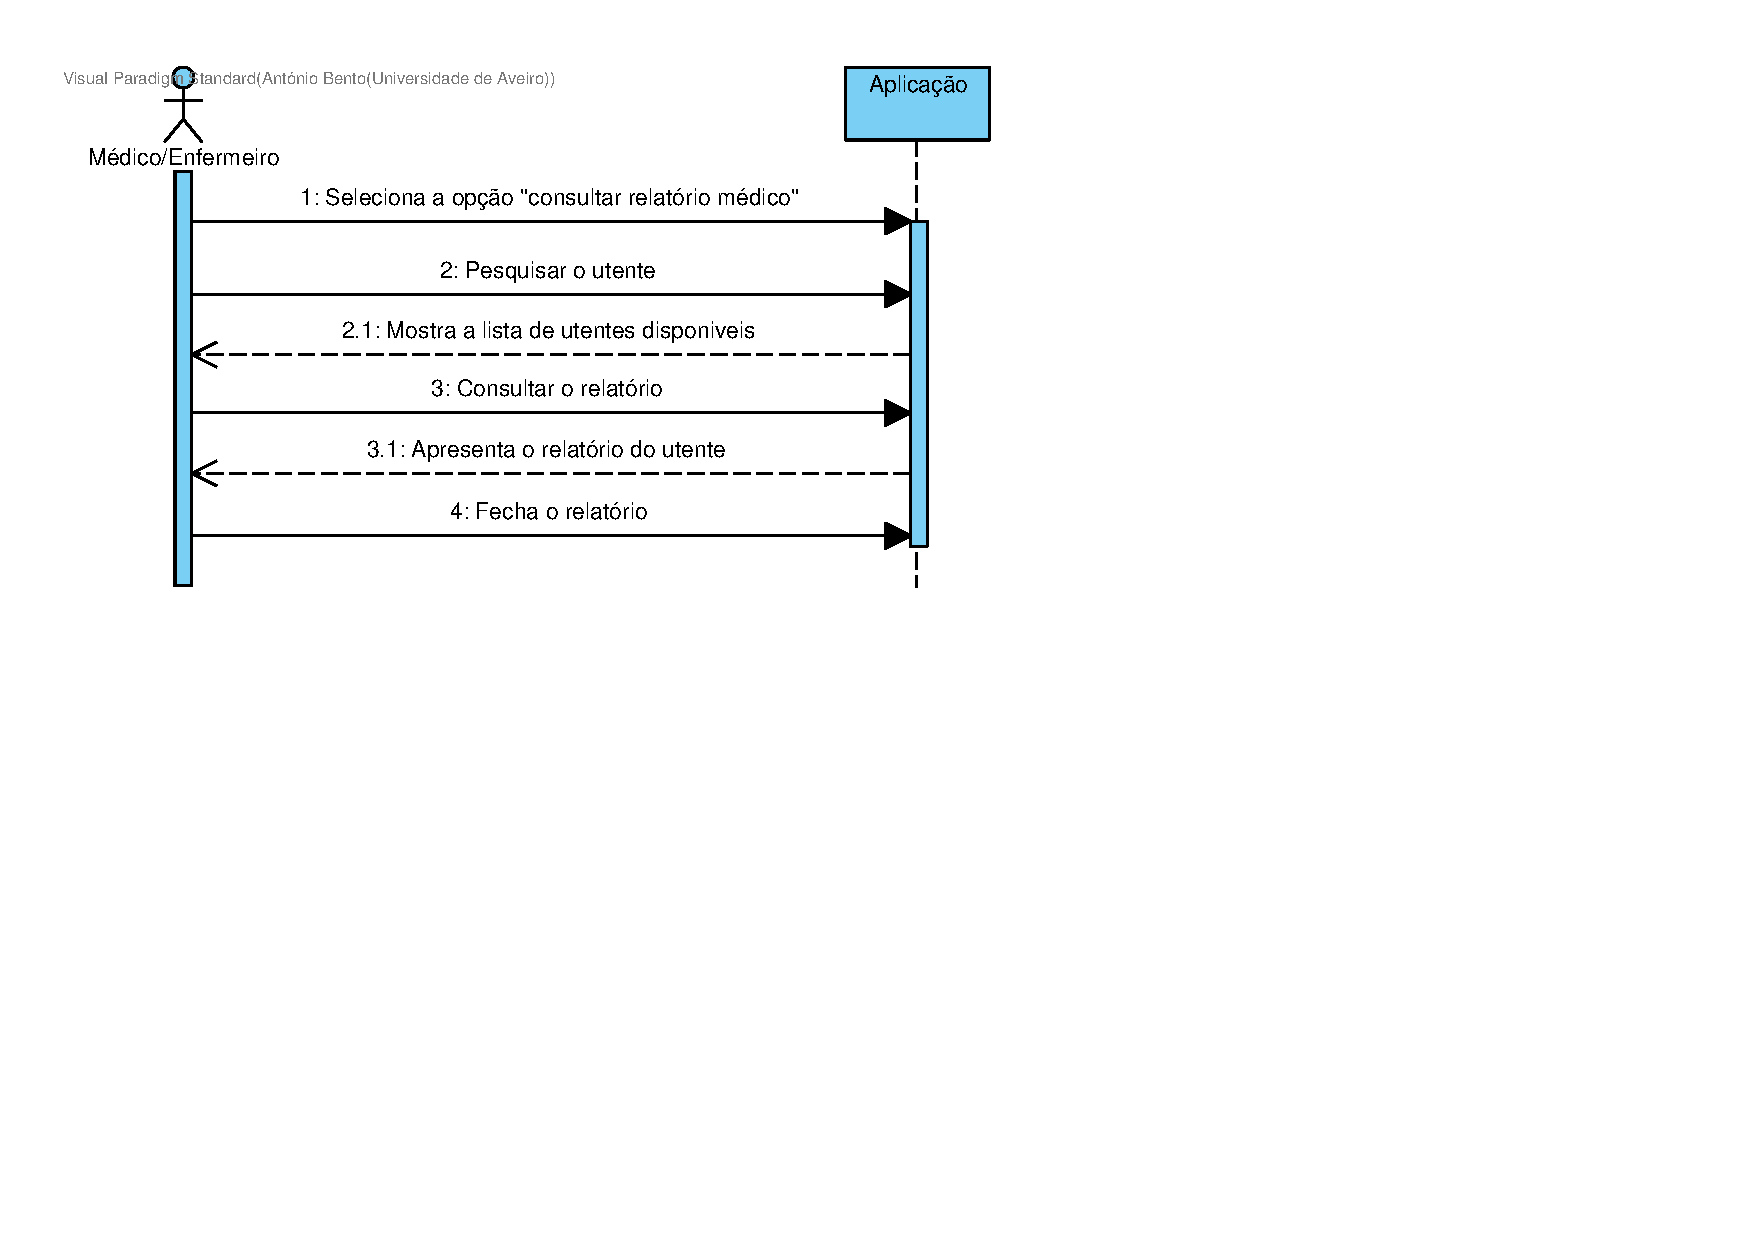
\includegraphics[width=0.7\linewidth]{image/Atividades/Consultar relatório}
	\caption{Diagrama de atividades - Consultar relatório médico do utente.}
	\label{fig:consultarrelatorio}
\end{figure}



\subsection{Consultar ficha do utente}

Após consulta, o utente solicita que lhe seja entregue uma justificação. O funcionário administrativo pesquisa pelo utente em questão, elaborando a justificação e entregando a mesma ao utente. 

\begin{center}
	\begin{tabularx}{\textwidth}{|lX|}
		\hline
		\textbf{Nome}: & \textbf{Consultar relatório médico do utente } \\ \hline
		Atores: & Médico e enfermeiro     \\ \hline
		Prioridade (1/3): & Alta  \\ \hline
		Finalidade: & Consultar informação presente na ficha de utente     \\ \hline
		Requisitos & RF.3, RF.4, RF.8   \\
		Funcionais: & \\
		Pré-condições: & Médico e/ou enfermeiro devem ter credenciais para aceder ao sistema \\
		Sumário: & O médico e o enfermeiro deverão introduzir as credencias, para depois poderem pesquisarem o utente e de seguida consultar a ficha de utente.  \\
		\hline
	\end{tabularx}
	
	\begin{tabularx}{\textwidth}{|XX|}
		\hline
		\multicolumn{2}{|c|}{\textbf{Sequência típica dos eventos} }\\
		\textbf{Ações dos atores}  & \textbf{Respostas do sistema} \\
		1.     O Profissional pesquisa o utente em questão   &   1.1 O sistema apresenta a lista de utentes   \\
		2.      O Profissional consulta a ficha de utente    & 2.1- O sistema apresenta a ficha referente ao utente selecionado     \\
		3.    O Profissional fecha a ficha de utente     &   \\
		\hline
		\multicolumn{2}{|c|}{\textbf{Sequências alternativas } }\\
		\hline
		\multicolumn{2}{|l|}{  }\\
		\hline
	\end{tabularx}
	
\end{center}

\begin{figure}[H]
	\centering
	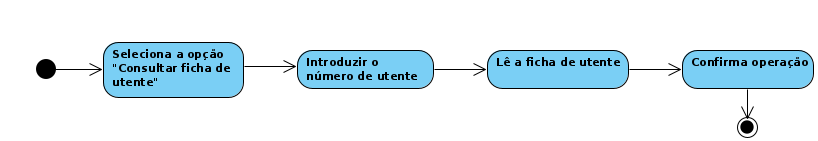
\includegraphics[width=0.7\linewidth]{image/Atividades/ConsultarFicha}
	\caption [Diagrama de atividades - Consultar ficha de utente.] {Diagrama de atividades - Consultar ficha de utente.}
	\label{fig:consultarfichautente}
\end{figure}


\subsection{Adicionar exames}

Em qualquer consulta, o médico pode requisitar a realização de exames. Tendo em consideração esta informação, o cliente, após a realização do exame, entra na consulta e entrega o exame ao médico ou enfermeiro que, de seguida, o introduzirá no sistema, dando a informação que o mesmo foi introduzido com sucesso. 

\begin{center}
	\begin{tabularx}{\textwidth}{|lX|}
		\hline
		\textbf{Nome}: & \textbf{Adicionar exames} \\ \hline
		Atores: & Médico, Enfermeiro    \\ \hline
		Prioridade (1/3): & Alta  \\ \hline
		Finalidade: & Adicionar uma descrição de um exame médico      \\ \hline
		Requisitos & RF.3, RF.13    \\
		Funcionais: & \\
		Pré-condições: & Médico e/ou enfermeiro devem ter credenciais para aceder ao sistema \\
		Sumário: & Adicionar ao relatório uma descrição de um exame médico  \\
		\hline
	\end{tabularx}
	
	\begin{tabularx}{\textwidth}{|XX|}
		\hline
		\multicolumn{2}{|c|}{\textbf{Sequência típica dos eventos} }\\
		\textbf{Ações dos atores}  & \textbf{Respostas do sistema} \\
		1.      O médico seleciona a opção para adicionar o exame    &   1.1- A interface apresenta o botão para adicionar exame médico   \\
		2.       O médico seleciona o ficheiro a importar     & 2.1-     A interface abre o explorador de ficheiros do sistema   \\
		3.      Utilizador carrega no botão de saída     & 3.1-     Importa o ficheiro para o sistema   \\
		& 3.2-     Envia o ficheiro para a base de dados \\
		&  3.3-   Associa o ficheiro ao relatório da consulta \\
		& 3.4-    Devolve mensagem de exportação concluída \\
		& 3.5-     Interface mostra botão de saída \\
		\hline
		\multicolumn{2}{|c|}{\textbf{Sequências alternativas } }\\
		\hline
		\multicolumn{2}{|l|}{ 1.1- Os médicos não têm a sessão iniciada no sistema e precisa de entrar na sua conta  }\\
		\multicolumn{2}{|l|}{ 3.1.1- O programa devolve mensagem de ficheiro inválido a ser importado  }\\
		\multicolumn{2}{|l|}{ 3.1.2- A importação falha ou é interrompida a meio }\\
		\multicolumn{2}{|l|}{3.2.1- Comunicação com a base de dados não ser possível  }\\
		\hline
	\end{tabularx}
	
\end{center}

\begin{figure}[H]
	\centering
	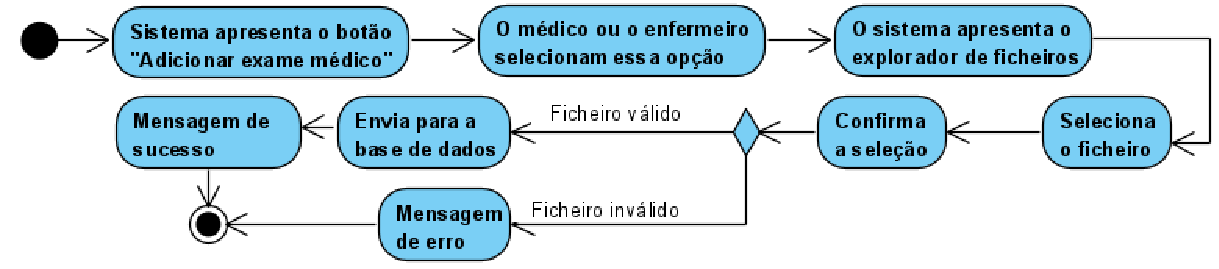
\includegraphics[width=0.7\linewidth]{image/Atividades/AdicionarExame}
	\caption [Diagrama de atividades - Adicionar exames.] {Diagrama de atividades - Adicionar exames.}
	\label{fig:adicionarexame}
\end{figure}


\subsection{Administrar medicação}

Depois da entrada do utente na consulta, foi necessário administrar medicação ao cliente. Para tal, o enfermeiro verifica a medicação a administrar e após a executar, registou em sistema o que foi administrado e por quem foi administrado.

\begin{center}
	\begin{tabularx}{\textwidth}{|lX|}
		\hline
		\textbf{Nome}: & \textbf{Administrar medicação } \\ \hline
		Atores: & Enfermeiro    \\ \hline
		Prioridade (1/3): & Alta  \\ \hline
		Finalidade: & Facilitar o processo de administração de medicação por parte do enfermeiro       \\ \hline
		Requisitos & RF.3, RF.12     \\
		Funcionais: & \\
		Pré-condições: & Enfermeiro deve ter credenciais para aceder ao sistema \\
		Sumário: & O enfermeiro dirige-se ao sistema com a sua sessão iniciada e consulta a ficha de utente. Lá terá uma opção para administrar medicação, que guardará essa informação.   \\
		\hline
	\end{tabularx}
	
	\begin{tabularx}{\textwidth}{|XX|}
		\hline
		\multicolumn{2}{|c|}{\textbf{Sequência típica dos eventos} }\\
		\textbf{Ações dos atores}  & \textbf{Respostas do sistema} \\
		1.    O enfermeiro consulta a ficha de utente    &   1.1     A interface apresenta a ficha de utente   \\
		2.    O enfermeiro seleciona a opção “Administrar Medicação”      & 2.1-   Interface apresenta um campo para inserção da medicação a administrar.   \\
		3.    O enfermeiro preenche esse campo e guarda a informação     & 3.1-   Dados guardados na base de dados   \\
		\hline
		\multicolumn{2}{|c|}{\textbf{Sequências alternativas } }\\
		\hline
		\multicolumn{2}{|l|}{} \\
		\hline
	\end{tabularx}
	
\end{center}


\begin{figure}[H]
	\centering
	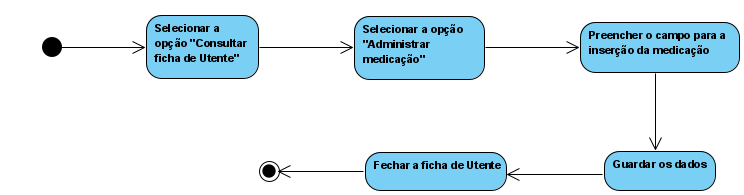
\includegraphics[width=0.7\linewidth]{image/Atividades/Administrar medicação.png}
	\caption [Diagrama de atividades - Administrar medicação.] {Diagrama de atividades - Administrar medicação.}
	\label{fig:administrarmedicacao}
\end{figure}


\section{Cobertura de requisitos}

\begin{figure}[H]
	\centering
	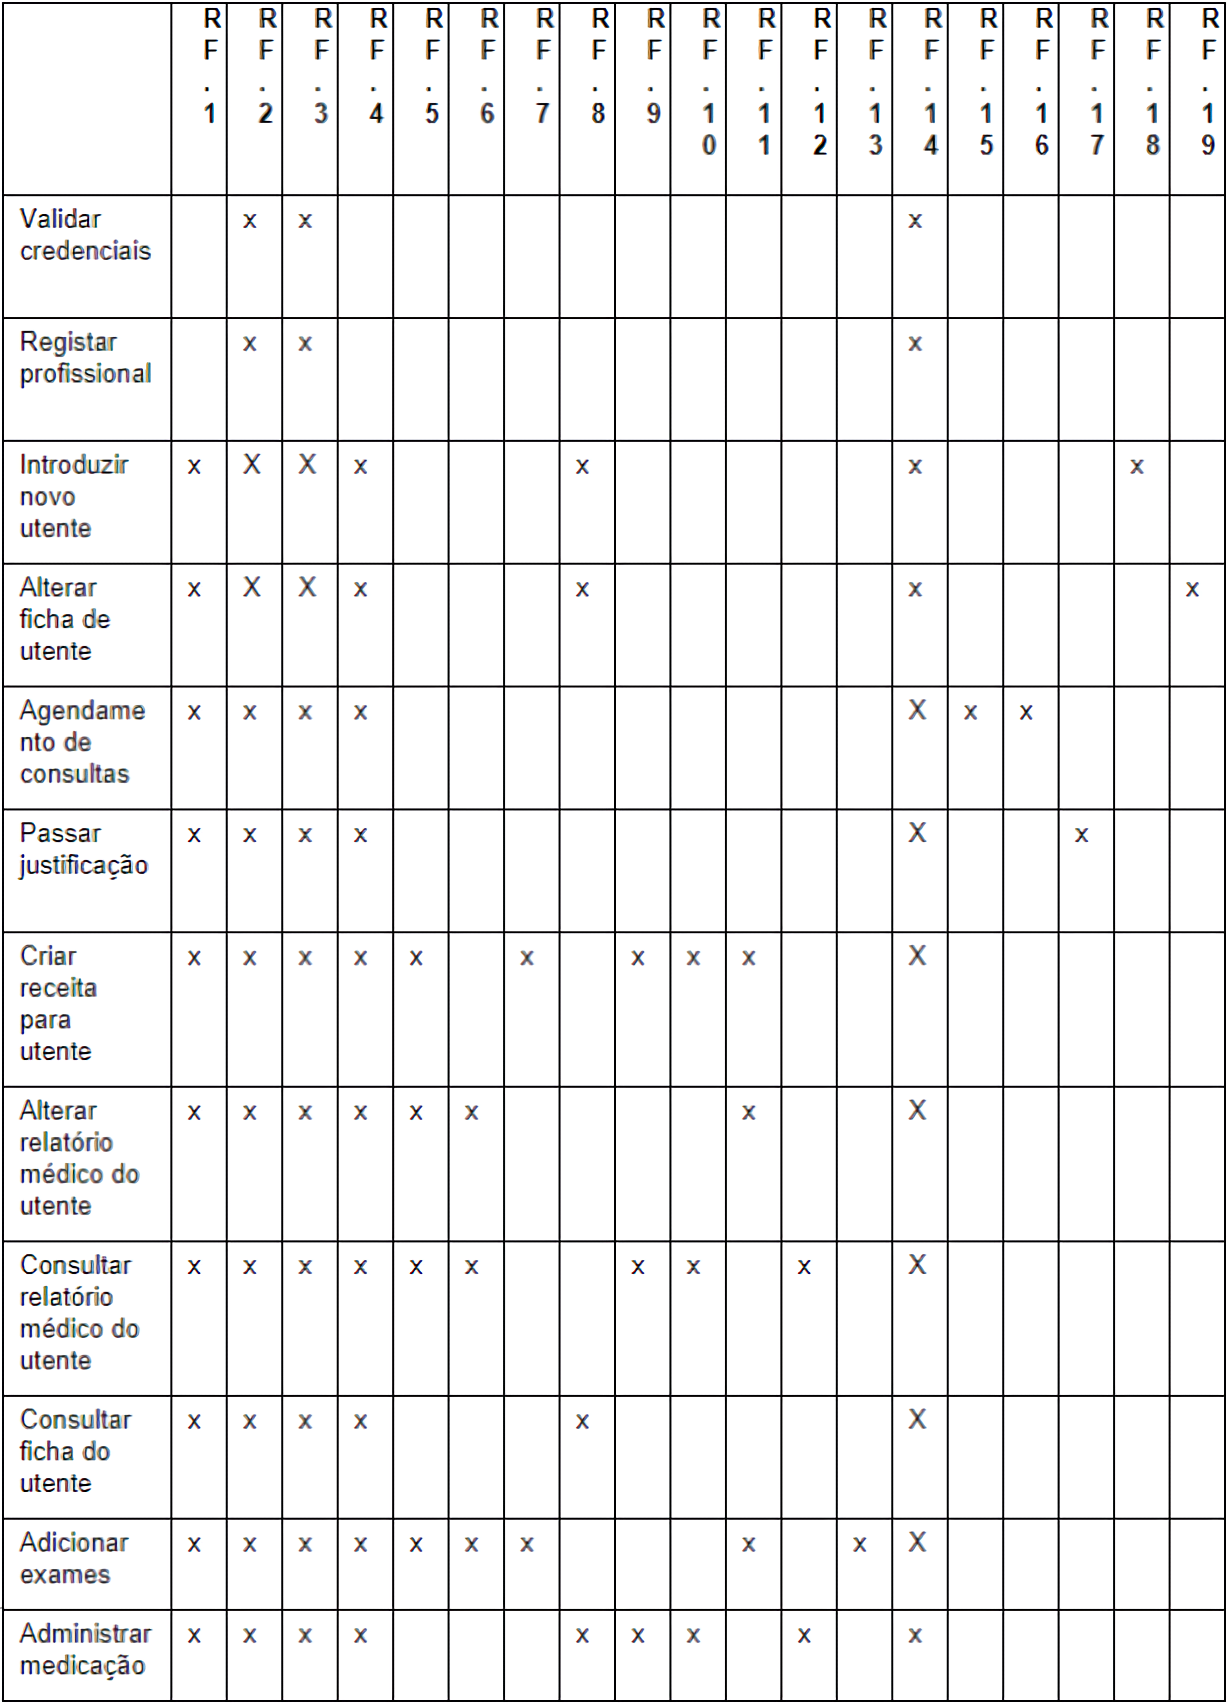
\includegraphics[width=0.9\linewidth]{image/CoberturaRequisitos2}
	\caption{Tabela de funcionalidades em função de requisitos.}
	\label{fig:coberturarequisitos}
\end{figure}


\chapter{Modelo de conceitos do domínio}

\begin{figure}[H]
	\centering
	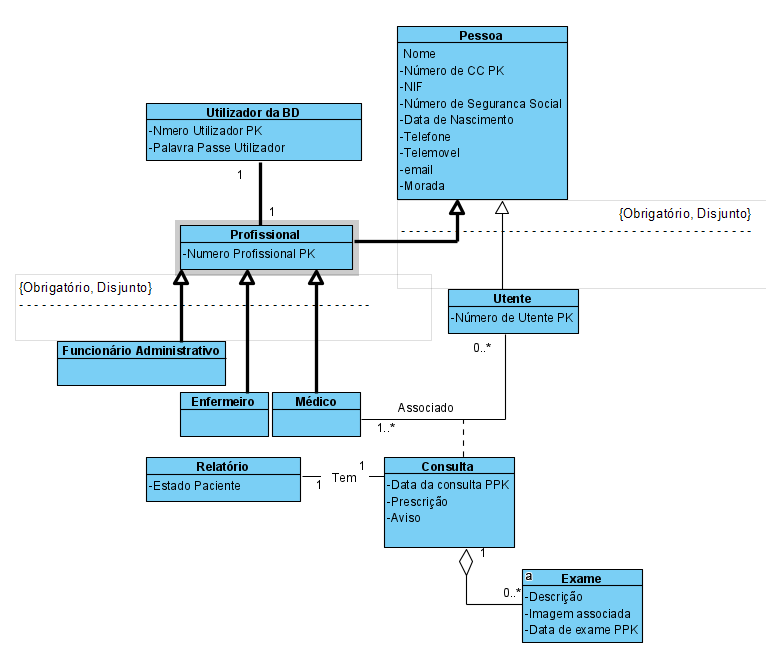
\includegraphics[width=0.95\linewidth]{image/DiagramaCLasses}
	\caption [Diagrama de Classes] {Diagrama de Classes}
	\label{fig:diagramaclasses}
\end{figure}

Após compreender os processos e intervenientes da clínica dentária, foi possível confirmar que tipologia terá o sistema no que toca à sua estrutura estática. Dito isto, foi elaborado um diagrama de classes que visa determinar todas as classes do sistema e os seus atributos, tal como se pode verificar na Figura \ref{fig:diagramaclasses}. 

Confirma-se a presença de relações na Figura \ref{fig:diagramaclasses}. Em primeiro lugar, o diagrama acima indicado foi elaborado tendo em conta quem interage com a aplicação e que tipos de interações existem entre estes e os utentes, permitindo descrever que atributos vão ser usados e onde são alojados, como por exemplo a relação existente entre médico e profissional, sendo que médico é uma especialização e profissional é uma generalização, também como, partindo do pressuposto, a consulta deriva da interação entre o médico e o cliente que por si tem um relatório e a qual cada cliente tem um e apenas um médico associado. 


\chapter{Especificação Lógica}

O objetivo principal foi desenvolver uma aplicação capaz de suportar o sistema de gestão de uma clínica dentária.
Tendo conhecimento da dimensão da equipa de desenvolvimento (6 elementos), ficou decidido que em cada semana todos os elementos se orientavam para um conjunto de requisitos específicos, permitindo organizar corretamente o trabalho. Foi também atribuído um \textit{project owner} a cada ciclo (1 semana) que contacta o cliente e apresentava, a cada ciclo o que foi desenvolvido pela equipa, usando assim um modelo ágil que se assemelha ao \textit{scrum}.
Foram concluídas fases iniciais do projeto tais como a fase da análise e definição de requisitos e o planeamento do sistema de desenvolvimento.

Os requisitos da clínica dentária foram definidos em maior parte aquando da análise do sistema e requisitos, sendo assim possível transitar para a fase de modelação e planeamento com grande parte das funcionalidades em consideração.
Em simultâneo com o planeamento, o cliente foi contactado sempre que necessário para qualquer orientação tendo sempre em atenção às necessidades do sistema. 

No que toca à estrutura de desenvolvimento, o grupo seguiu as indicações do \textit{project owner}, sendo que este elaborou o \textit{sprint backlog} que contém as necessidades a ser implementadas para cada \textit{sprint}.
A equipa organizou-se de modo a que cada elemento recebesse tarefas com responsabilidade, carga horária e grau de dificuldade semelhantes. 
O objetivo predominante nas fases iniciais foi preparar o ambiente para cada elemento e foram tomadas decisões como o \textit{software} de desenvolvimento e \textit{software} de controlo de versões.
Dito isto, são enumeradas as seguintes decisões: 

\begin{itemize}
	\item \textit{Software} de controlo de versões: Git 
	\item Servidor para controlo de versões: GitHub 
	\item Sistema de gestão de base de dados: MySQL com MySQL WorkBench
\end{itemize}


Com o objetivo de obter uma boa estrutura de desenvolvimento tomou-se a decisão de usar o mesmo \textit{software} em todas as máquinas de desenvolvimento da aplicação; 


\begin{itemize}
	\item IDE para desenvolvimento em Python: Atom, PyCharm, Sublime, Spyder, VSCode e CLI. 
	\item \textit{Framework} de desenvolvimento de interface gráfica: QtDesigner 
	\item \textit{Software} de desenvolvimento de documentação formal: \LaTeX \hspace{0.1cm}com TexStudio 
\end{itemize}


\chapter{Modelo dinâmico}

%\section{Funções de sistema}

Aqui vamos apresentar todas as funcionalidades relacionadas com o ator que as executa. Existem também certas funcionalidades que estão interligadas entre si. 


\section{Validação de Credenciais }

\begin{figure}[H]
	\centering
	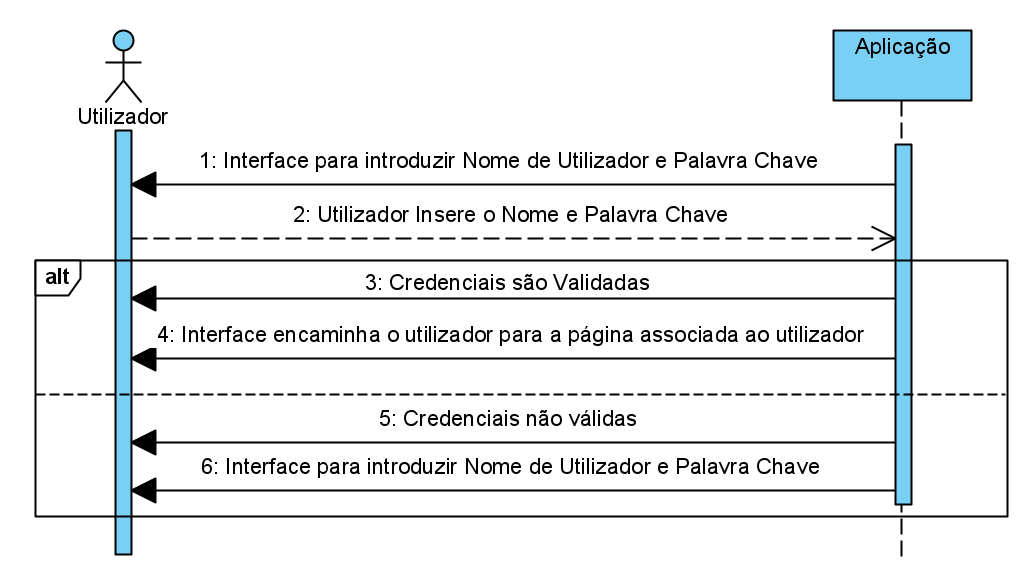
\includegraphics[width=0.7\linewidth]{image/SequencialDiagramsImages/Validar_credenciais}
	\caption [Diagrama de sequências de validação de credenciais.] {Diagrama de sequências de validação de credenciais.}
	\label{fig:validarcredenciaisF}
\end{figure}

A validação de credenciais dá-se para todos os utilizadores do sistema.
É um caso importante pois permite e/ou delimita as funcionalidades que cada utilizador possa fazer. 

\section{Registar Profissional}

\begin{figure}[H]
	\centering
	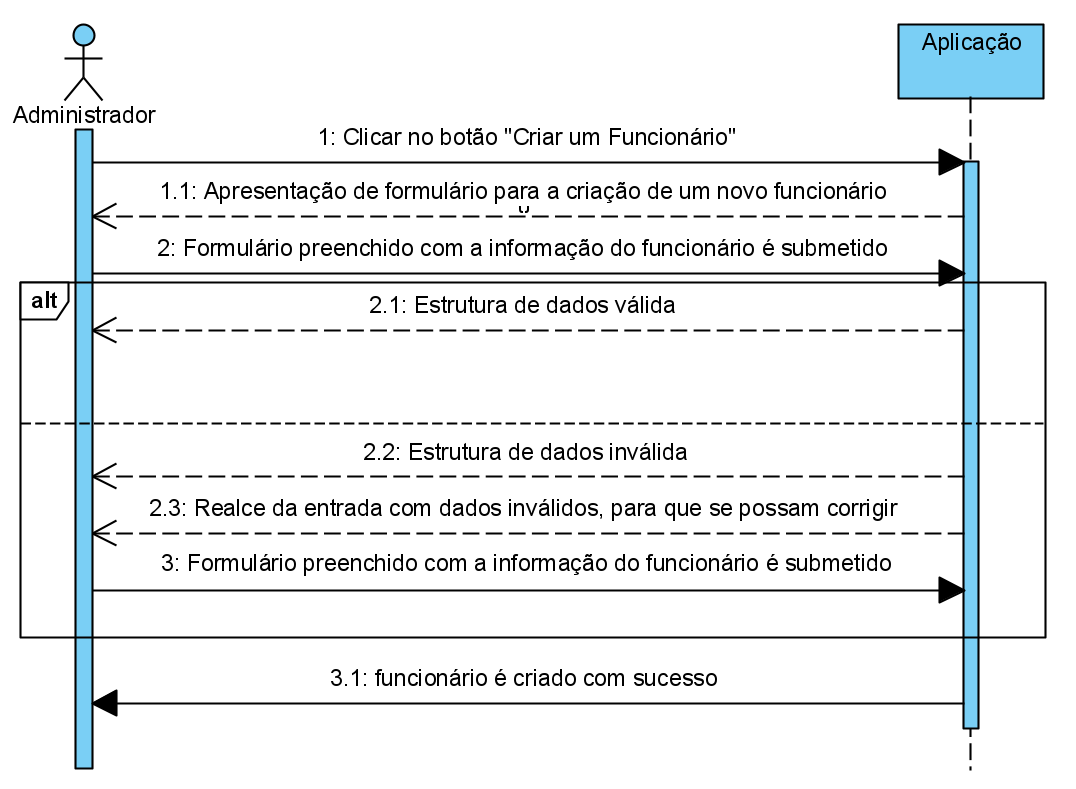
\includegraphics[width=0.7\linewidth]{image/SequencialDiagramsImages/Registar_pessoal}
	\caption [Diagrama de sequências de registar profissional.] {Diagrama de sequências de registar profissional.}
	\label{fig:registarpessoalF}
\end{figure}

Esta função é exclusiva para o administrador do sistema.
Serve para adicionar profissionais ao sistema, como médicos, funcionários administrativos e enfermeiros, que fará uma atribuição de permissões para com a conta do utilizador. 

\section{Introduzir novo utente}

\begin{figure}[H]
	\centering
	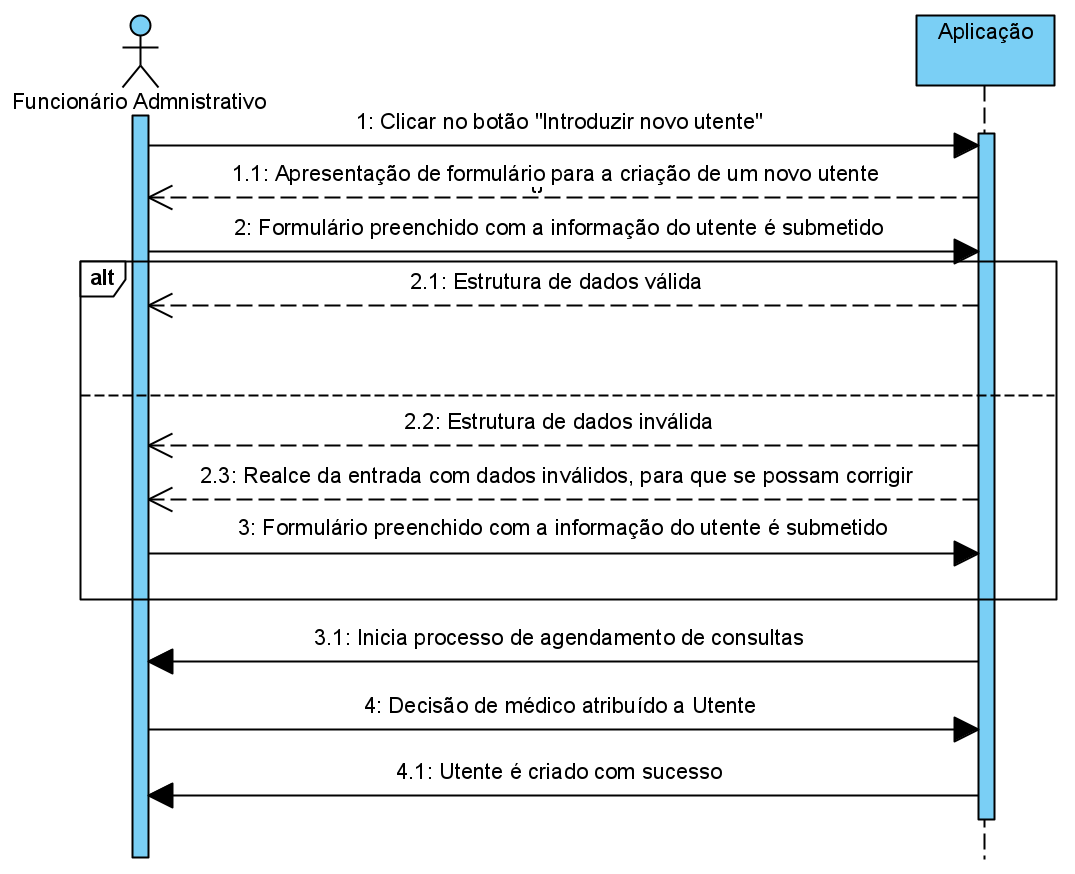
\includegraphics[width=0.7\linewidth]{image/SequencialDiagramsImages/Introduzir_novo_utente}
	\caption [Diagrama de sequências de introduzir novo utente.] {Diagrama de sequências de introduzir novo utente.}
	\label{fig:introduzirnovoutenteF}
\end{figure}

A introdução de um novo utente é feita pelo funcionário administrativo.
Este processo serve para fazer a criação de um novo utente para que todos os seus dados fiquem guardados na base de dados e para que se possa criar a respetiva ficha. 

\section{Alterar Ficha de Utente}

\begin{figure}[H]
	\centering
	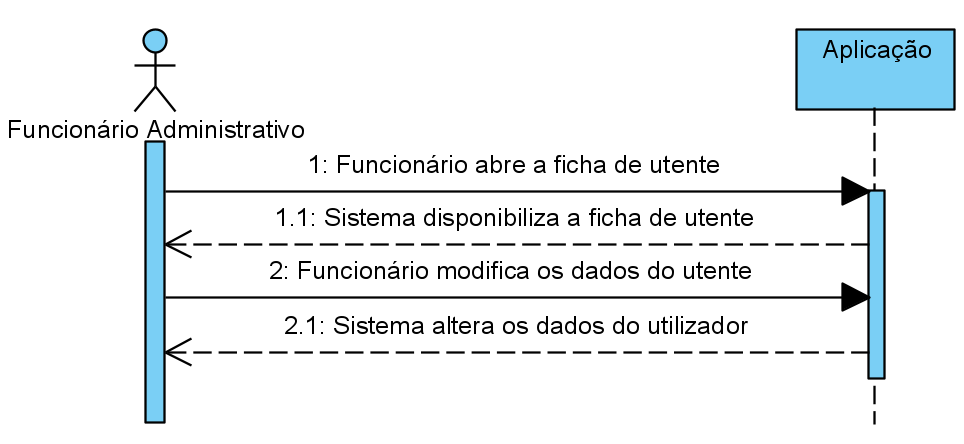
\includegraphics[width=0.7\linewidth]{image/SequencialDiagramsImages/Alterar_ficha_utente}
	\caption [Diagrama de sequências de alterar ficha de utente.] {Diagrama de sequências de alterar ficha de utente.}
	\label{fig:alterarfichautenteF}
\end{figure}

Esta função é usada pelo funcionário administrativo e serve para a alteração de dados na ficha de utente, quando necessário.

\section{Agendamento de Consultas }


\begin{figure}[H]
	\centering
	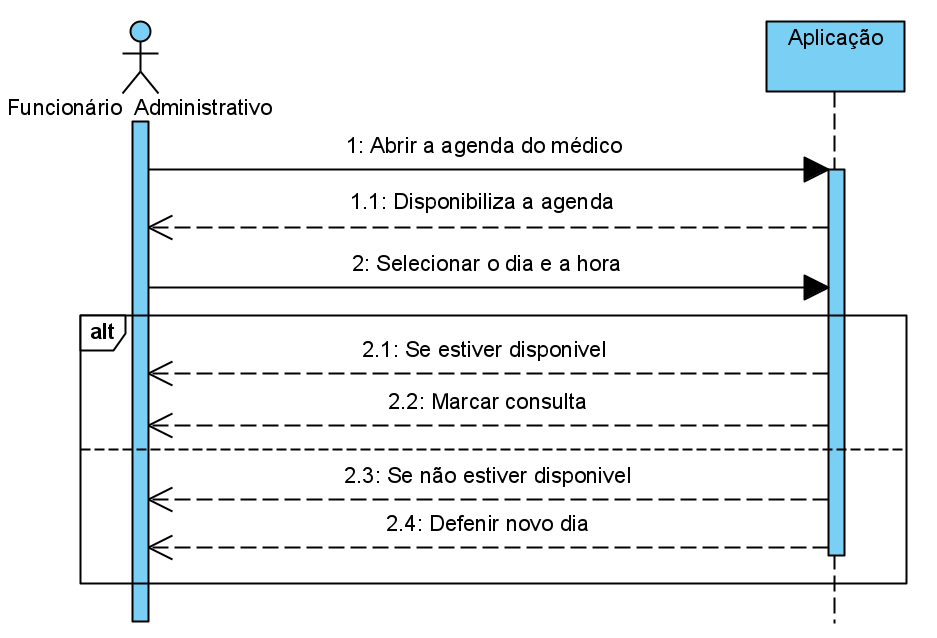
\includegraphics[width=0.7\linewidth]{image/SequencialDiagramsImages/Agendamento_consultas}
	\caption [Diagrama de sequências de agendamento de consultas.] {Diagrama de sequências de agendamento de consultas.}
	\label{fig:agendamentoconsultasF}
\end{figure}

A funcionalidade poderá ser utilizada pelo funcionário administrativo.
Tem como objetivo a marcação de uma consulta num determinado dia e hora. 

\section{Passar Justificação}

\begin{figure}[H]
	\centering
	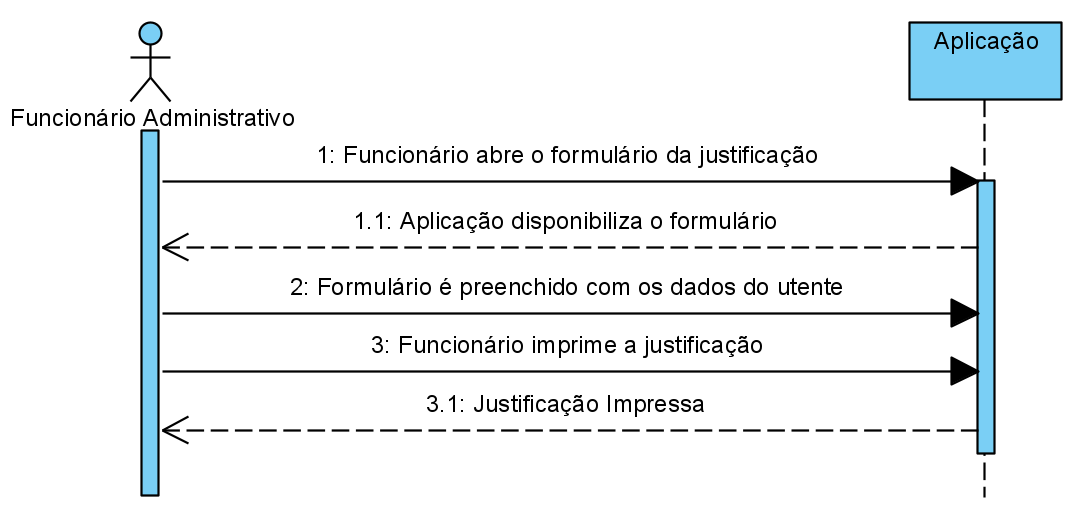
\includegraphics[width=0.7\linewidth]{image/SequencialDiagramsImages/Passar_justificação}
	\caption [Diagrama de sequências de passar justificação.] {Diagrama de sequências de passar justificação.}
	\label{fig:passarjustificacaoF}
\end{figure}

Esta função será apenas utilizada pelo funcionário administrativo. Tem como objetivo criar um comprovativo de como o utente esteve de facto numa consulta. 


\section{Criar Receita}

\begin{figure}[H]
	\centering
	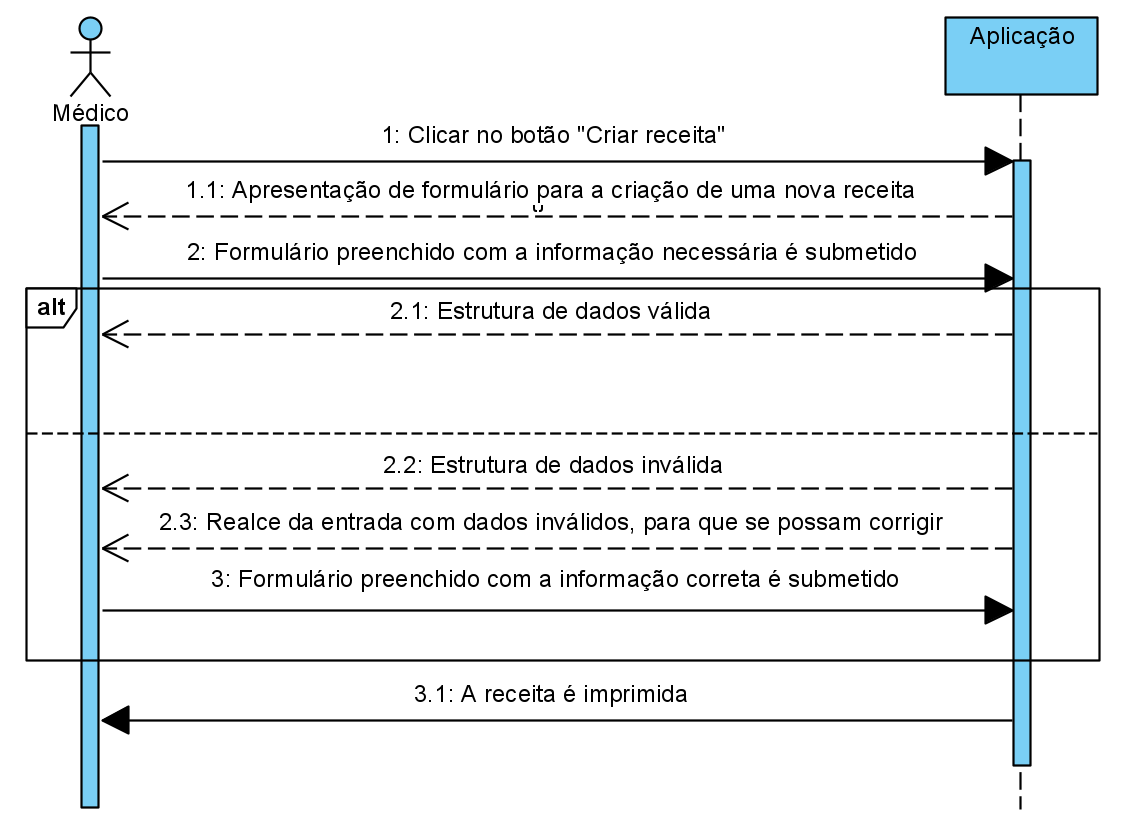
\includegraphics[width=0.7\linewidth]{image/SequencialDiagramsImages/CriarReceita}
	\caption [Diagrama de sequências de criar receita.] {Diagrama de sequências de criar receita.}
	\label{fig:criarreceitaF}
\end{figure}

Esta função será utilizada pelo médico e o funcionário administrativo. Em que o médico com ela cria uma receita para o utente, para que este possa comprar o medicamento nela descrito numa farmácia. E o funcionário administrativo imprime a receita e entrega-a ao utente. 

\section{Alterar Relatório Médico do Utente }

\begin{figure}[H]
	\centering
	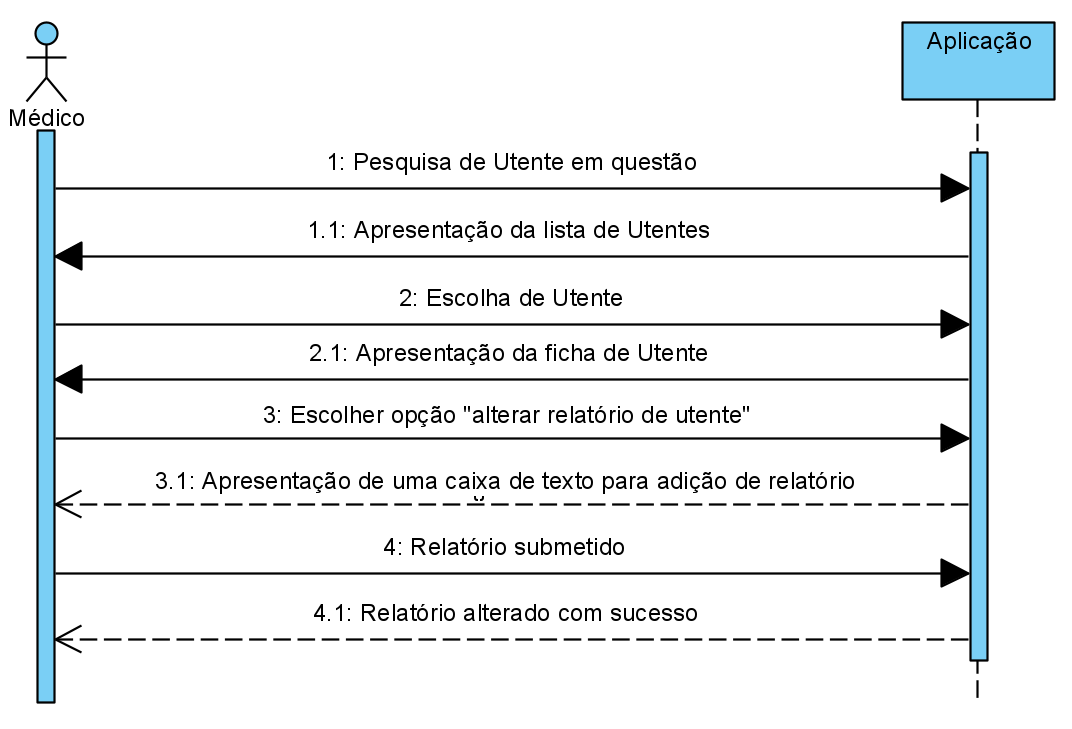
\includegraphics[width=0.7\linewidth]{image/SequencialDiagramsImages/AlterarRelatórioMédico}
	\caption [Diagrama de sequências de alterar relatório médico do utente.] {Diagrama de sequências de alterar relatório médico do utente.}
	\label{fig:alterarrelatoriomedicoF}
\end{figure}

A função mencionada apenas poderá ser utilizada pelo médico.
Com esta, o médico altera ou acrescenta informação ao relatório médico em questão. 


\section{Consultar Relatório Médico do Utente }


~\begin{figure}[H]
	\centering
	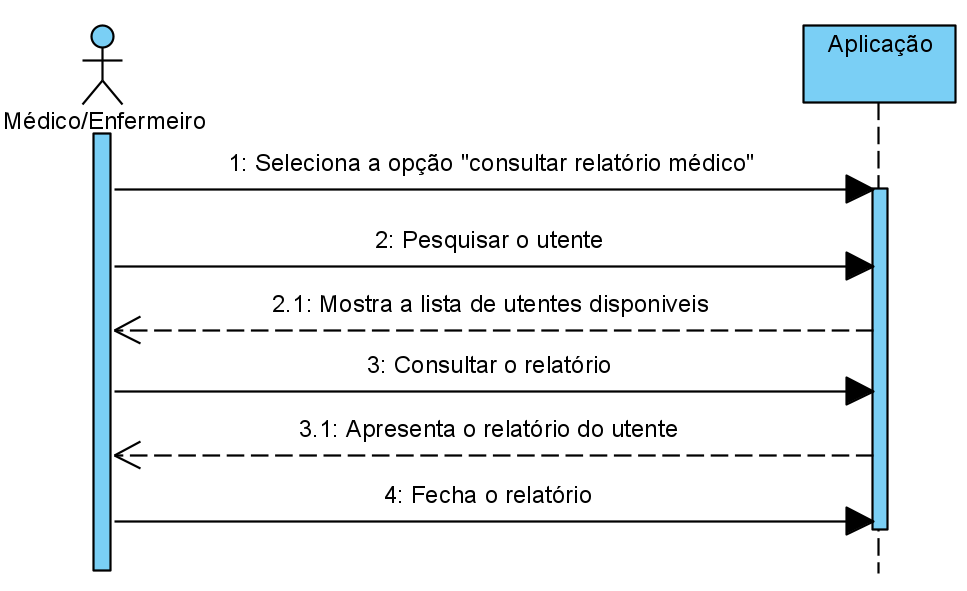
\includegraphics[width=0.7\linewidth]{image/SequencialDiagramsImages/Consultar_relatorio}
	\caption [Diagrama de sequências de consultar relatório médico do utente.] {Diagrama de sequências de consultar relatório médico do utente.}
	\label{fig:consultarrelatorioF}
\end{figure}

A função presente pode ser utilizada pelo médico e pelo enfermeiro. Com esta, os atores podem consultar o relatório médico para consultar as suas informações.

\section{Consultar Ficha de Utente }

\begin{figure}[H]
	\centering
	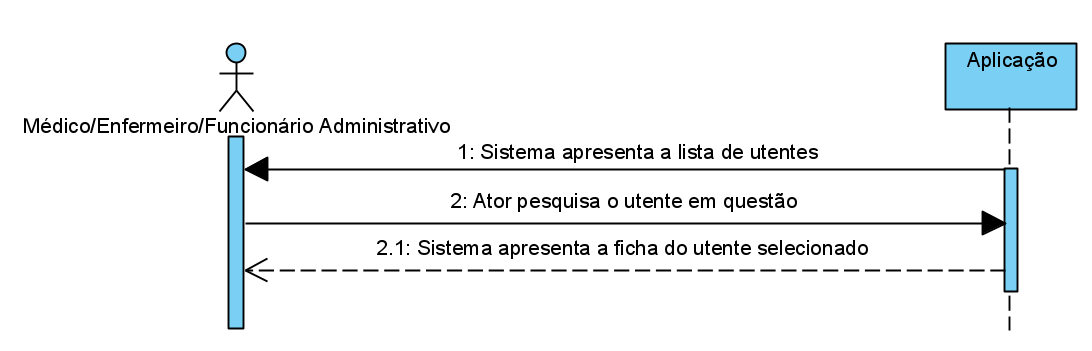
\includegraphics[width=0.7\linewidth]{image/SequencialDiagramsImages/Consultar_ficha_utente}
	\caption [Diagrama de sequências de consultar ficha do utente.] {Diagrama de sequências de consultar ficha do utente.}
	\label{fig:consultarfichautenteF}
\end{figure}

A funcionalidade poderá ser utilizada pelo médico, enfermeiro e funcionário administrativo. 
Tem como objetivo consultar a ficha de utente, para aceder tanto aos dados pessoais como aos dados de consultas anteriores (que estão guardadas nos relatórios médicos). 

\section{Adicionar Exames}

\begin{figure}[H]
	\centering
	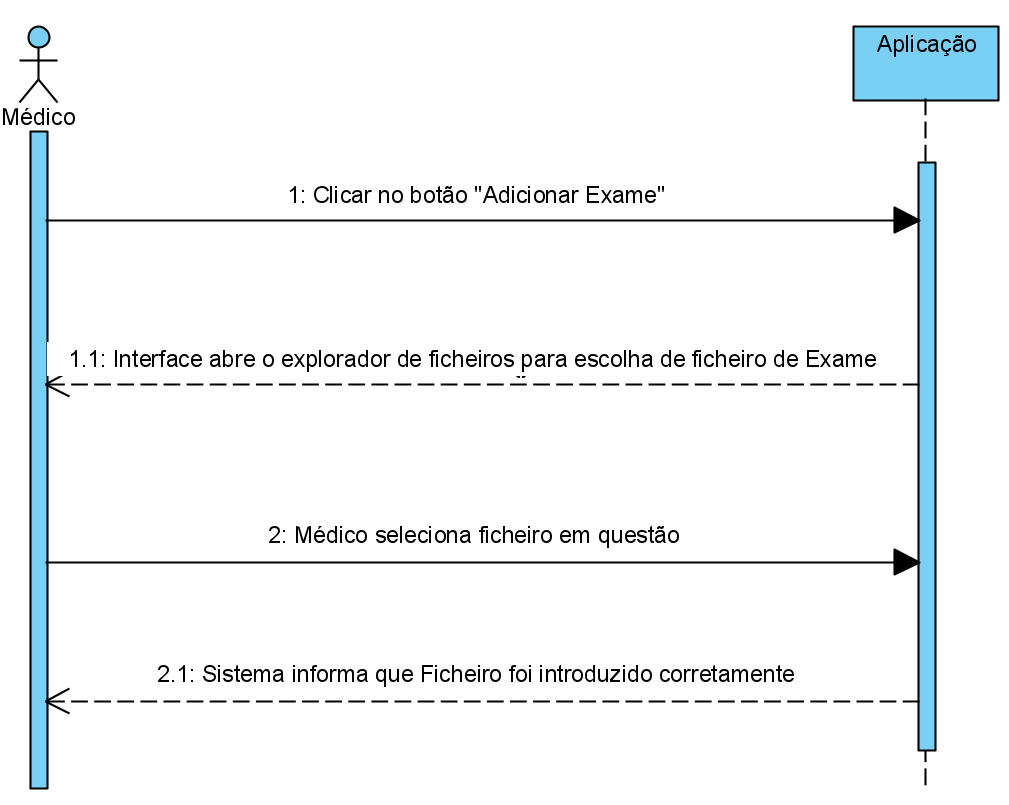
\includegraphics[width=0.7\linewidth]{image/SequencialDiagramsImages/AdicionarExame}
	\caption [Diagrama de sequências de adicionar exames.] {Diagrama de sequências de adicionar exames.}
	\label{fig:adicionarexameF}
\end{figure}

Esta função poderá ser utilizada pelo médico e pelo enfermeiro. Consiste em adicionar um exame ao relatório médico do utente. 


\section{Administrar Medicação }

\begin{figure}[H]
	\centering
	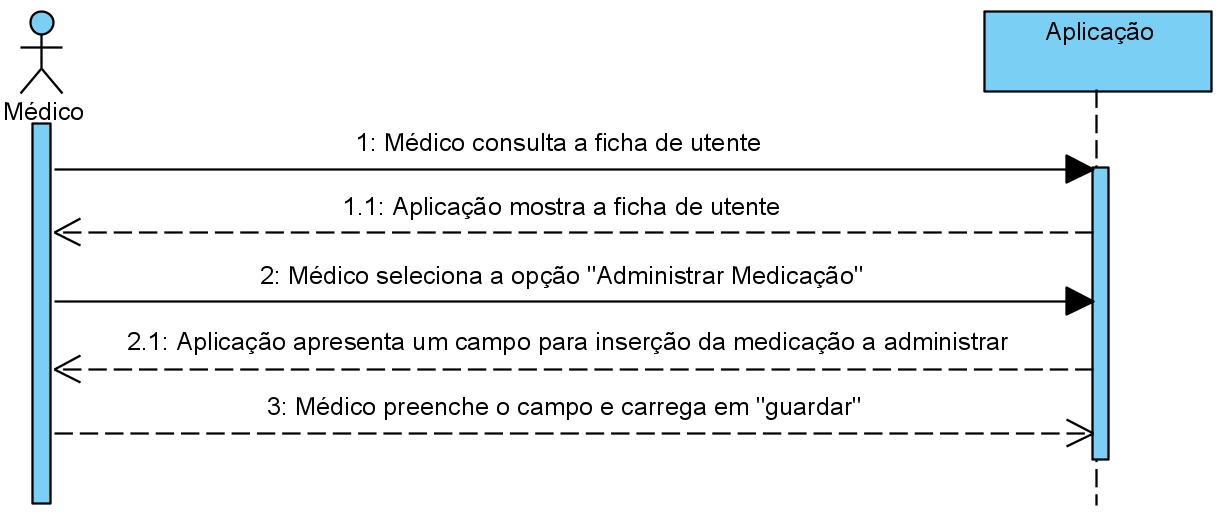
\includegraphics[width=0.7\linewidth]{image/SequencialDiagramsImages/AdministrarMedicação}
	\caption [Diagrama de sequências de administrar medicação.] {Diagrama de sequências de administrar medicação.}
	\label{fig:administrarmedicacaoF}
\end{figure}

A funcionalidade aqui descrita é utilizada pelo enfermeiro e consiste em guardar no relatório médico o que foi administrado e por quem foi administrado durante a consulta. 


%\section{Colaborações entre objetos }
%
%Existem certas funcionalidades que estão diretamente ligadas entre si.
%Entre estas, a mais importante é Validar Credenciais, que acontece assim que o utilizador faz o \textit{Login} na máquina, que por sua vez dará ao utilizador todas as permissões que necessita para executar as respetivas tarefas. 
%
%Existem também vários casos de consulta que estão diretamente relacionados com casos de alteração de dados: 

\begin{itemize}
	\item     Consultar e Alterar relatório médico.
	\item     Consultar e Alterar ficha de utente.
\end{itemize}

\chapter{Modelo de dados persistente}

Dados os requisitos estabelecidos e a divisão lógica do modelo conceptual, foi realizada a transposição para o seguinte modelo de dados persistentes:

\begin{itemize}
	\item   utente (nome \{not null\}, nr\_cartao\_cidadao \{not null, unique\}, nif \{not null, unique\}, nr\_seg\_social \{not null, unique\}, data\_nascimento \{not null\}, telefone, telemovel \{not null\}, email, morada \{not null\}, \underline{numero\_utente}, ativo \{not null\})
	
	\item	id\_funcionario (nome \{not null\}, nr\_cartao\_cidadao \{not null, unique\}, nif \{not null, unique\}, nr\_seguranca\_social \{not null, unique\}, data\_nascimento \{not null\}, telefone \{not null\}, telemovel \{not null\}, email \{not null\}, morada \{not null\}, \underline{funcionario\_numero}, profissao \{not null\}, ativo \{not null\})
	
	\item	funcionario (\underline{numero}, utilizador\_nome \{not null\}, palavra\_passe \{not null\}, secret\_key \{not null\})
	
	\item	consulta (\underline{data}, \underline{utente\_numero}, relatorio\_consulta \{not null\}, funcionario\_numero \{not null\}, aviso\_consulta, hora \{not null\}, medicacao\_administrada, prescricao\_consulta)
	
	\item	exame(\underline{ID}, \underline{consulta\_data}, \underline{consulta\_utente\_numero}, data\_exame \{not null\}, imagem\_exame \{not null\}) \\
\end{itemize} 
	
	Este modelo de dados presistente, contém as relações necessárias que a base de dados irá conter, respetivamente com os seus atributos, em que os atributos que estão sublinhados designam-se por chave primária de cada relação. E sempre que um atributo é seguido de "not null", significa que o mesmo não pode estar vazio, ou seja, deve conter sempre alguma informação. Se o atributo for seguido de "unique", significa que a informação deste atributo é única e que não pode ser repetida.\\






\chapter{Código e Design}

	Embora exista uma clara distinção entre o código e a interface do utilizador, ambos foram desenvolvidos em paralelo de modo a permitir um ambiente de desenvolvimento útil para \textit{debugging}.
	
	Dada a divisão de profissões dentro da clínica, a equipa de desenvolvimento decidiu dividir os ficheiros de sistema de acordo com a profissão em causa, para que fosse possível um nível de controlo significativo sobre as funcionalidades de cada utilizador, mesmo assim, existe ainda uma divisão lógica caracterizada pela distribuição de código associado a tarefas diferentes por cada ficheiro, como por exemplo o "Connection.py" que alberga código orientado para alterar variáveis no âmbito da conexão à base de dados.	

\section{Programação}
	
	\subsection{Planeamento}
	
	Em primeiro lugar, é necessário ter as seguintes ideias em mente, o projeto é dividido em vários ficheiros, nomeadamente organizados por funcionalidade ou classe associada à profissão do utilizador, existe a necessidade de ter uma estrutura coesa que ligue a interface ao código funcional que contacta com a base de dados, cada elemento do grupo é responsável por uma parte considerável do produto final, de modo a distribuir responsabilidade irmãmente pelos membros da equipa.
	
	
	\subsection{Preparação}
	
	Tendo em conta os conceitos descritos anteriormente, foi decidido utilizar um sistema de controlo de versões capaz de monitorizar e gerir o trabalho realizado, tendo em conta as dimensões do projeto e a utilidade da aplicação o git foi estabelecido como plataforma de controlo de versões, na qual existe uma ligação ao GitHub que permite um controlo eficaz e constante do desenvolvimento do projeto.
	
	
	\subsection{Desenvolvimento}
	
	Numa fase inicial foi estipulado elaborar um ficheiro de testes (Index(.py)) para que sejam adicionadas e alteradas funcionalidades aquando necessário, associado a este foi elaborada uma interface de testes designada por Index(.ui), ambos permitiram suportar o desenvolvimento de novas funcionalidades, que mais tarde foram migradas para os respetivos ficheiros.
	
	Pondo a relação dos ficheiros de um modo lógico, o ficheiro principal a ser executado denomina-se main(.py), este é responsável por validar o \textit{login} de utilizadores e chamar corretamente a interface/código associado à profissão registada.
	
	Dado que foram elaborados ficheiros para cada tipo de profissão, cada um destes inicia uma interface individualmente, possibilitando a correta separação de funcionalidades e ecrãs pelos diferentes tipos de utilizadores de sistema.
	Existem 4 interfaces distintas, estas sendo:
	\begin{itemize}
		\item Administrador
		\item Médico
		\item Enfermeiro
		\item Rececionista
	\end{itemize}

	As funcionalidades de cada interface apresentada correspondem diretamente às indicadas na Figura \ref{fig:DiagramaCasoUso}.
	
	Os contactos com a base de dados são uma componente fundamental para o correto funcionamento do sistema permitindo que sejam introduzidos, consultados, ou alterados dados da base de dados, estes contactos foram realizados estabelecendo uma ligação que é caraterizada, nomeadamente, pelos conteúdos do ficheiro Connection(.py).
	
	Foi tomada em consideração a necessidade de terminar todas as chamadas com a base de dados assim que estas se tornem desnecessárias, podendo assim aceder com várias instâncias do programa abertas.
	
	Algumas funcionalidades requerem ser apresentadas com melhor detalhe para que se entendam "os porquês" de estarem assim desenvolvidas, tal como a funcionalidade de apresentar justificação que de momento apresenta um pop-up, isto é justificado sendo que no ambiente em que o programa vai ser usado, existem impressoras com uma ligação direta ao sistema permitindo que a justificação seja automaticamente impressa, como no ambiente de desenvolvimento não existia tal aparelho, quando se passa uma justificação para determinada consulta esta apenas emite um pop-up. 
	
	Existe também a funcionalidade de registar e apresentar um exame, este exame pode ser guardado nos formatos (.png), (.jpeg) e (.pdf), foram selecionados estes tipos de ficheiro porque considerou-se que seriam mais relevantes e próximos da realidade possível, ao selecionar um exame existente este é apresentado (no respetivo campo designado do ecrã para apresentar exames) caso seja de formato (.png) e (.jpeg), caso seja um ficheiro do tipo (.pdf) este é enviado para o ambiente de trabalho, esta funcionalidade foi desenvolvida desta forma porque os ficheiros (.pdf) podem conter várias páginas e não seria possível apresentar do mesmo modo que os outros formatos são apresentados.
	
	O agendamento de consultas e a introdução de dia e hora do mesmo é validado através de código em Python, isto porque o grupo decidiu que seria correto o utilizador não conseguir selecionar dias inválidos, pelo qual desenvolver esta funcionalidade apenas podia ser feita diretamente no código, tendo isto em conta, o calendário não permite a entrada de dias inválidos prevenindo a introdução de datas incorretas.
	
	Depois de estarem concluídas várias funcionalidades e de todos os elementos da equipa estarem familiarizados com as mesmas, nomeadamente consultar ficha de utente, analisar consulta, adicionar editar funcionários entre outras, começou-se a divisão lógica para ficheiros respetivos à tipologia do utilizador, foram então criados 4 ficheiros correspondentes aos 4 tipos de utilizadores presentes na clínica, sendo estes os médicos, enfermeiros, rececionistas e administradores de sistema.
	
	Para cada ficheiro foram tomadas abordagens diferentes visto que cada utilizador tem diferentes tipos de acesso à mesma informação, como por exemplo a forma como se acede à lista de consultas, que tanto pode ser feita a partir da ficha de utente, como pode ser feita a partir da aba de consultas associadas ao médico (funcionalidade apenas possível para o médico).
	
	Dando importância à necessidade de apresentar ao utilizador quem está registado na aplicação, foi desenvolvido um pequeno painel que apresenta os dados do utilizador com sessão iniciada no momento, este painel apresenta o nome e número do utilizador, foi tomada a decisão de o colocar este painel sempre visível atendendo aos princípios de consistência na apresentação da aplicação.
	
	\subsubsection{Médico}
	O ficheiro que contém as funcionalidades inerentes ao médico é denominado por medicWindow(.py) e encontra-se em PyClinic/classes/, o ficheiro respetivo à interface do médico denomina-se por medicWindow(.ui) e encontra-se em PyClinic/UI/.
	
	Na divisão de ficheiros, foi transitado código correspondente às atividades do médico do Index(.py) para o medicWindow(.py), nomeadamente foram transitadas funcionalidades como apresentar a tabela de utentes, de 
	consultas, a capacidade de analisar a consulta e a possibilidade de editar os dados de utilizador, a partir deste momento foram construidas funcionalidades que apenas dizem respeito ao médico tais como a capacidade de alterar o relatório, a prescrição, avisos da consulta e ainda adicionar exames e analisar exames.
	
	Particularmente no desenvolvimento da interface do médico, foi decidido que o médico necessitava de ter a capacidade de saber que consultas estavam atribuídas ao mesmo, ora com isto foi desenvolvida uma aba especifica para o mesmo que, dependendo do número que identifica o médico, apresenta todas as consultas que este tem da mais recente para a mais antiga.
	
	O grupo decidiu que seria útil se as consultas tivessem um campo de aviso, então foram desenvolvidos 2 campos no ecrã de apresentação da consulta, estes campos são designados por "Avisos" e "Avisar para a próxima consulta", estes campos apresentam os avisos para a consulta atual e os avisos a apresentar na próxima consulta respetivamente.
	
	Por questões de regulamentação, foi debatido em grupo se o médico ou qualquer outro utilizador poderia alterar os conteúdos da consulta após a mesma estar realizada ou antes desta acontecer, decidiu-se que por uma questão de lei, só o médico pode alterar o relatório, prescrição e avisos de consulta, e só o pode fazer no dia para que a consulta está agendada, impedindo que fraudes sejam cometidas ao tentar alterar estes dados fora do seu tempo designado.
	
	Tendo em conta que para cada consulta podem existir vários exames, foi desenvolvido uma aba reservada apenas para os mesmos, onde é possível consultar todos os exames associados ao utente, o mesmo foi desenvolvido desta forma para que o médico possa comparar facilmente um exame com outro sendo que ambos podem ser mostrados sequencialmente no mesmo ecrã.
	
	Foi colocado um painel na parte inferior do ecrã que apresenta as mensagens de sucesso quando a atualização da base de dados é efetuada corretamente, este painel foi desenvolvido sendo que o grupo de desenvolvimento considerou necessário apresentar ao utilizador informação atualizada sobre o estado do sistema, permitindo assim que o utilizador obtenha um \textit{feedback} da aplicação sempre que efetua uma ação de alteração na base de dados.
	
	\subsubsection{Enfermeiro}
	O ficheiro que contém as funcionalidades inerentes ao enfermeiro tem o nome nurseWindow(.py) encontrado em PyClinic/classes/, o ficheiro de UI referente ao enfermeiro denomina-se nurseWindow(.ui) e encontra-se em PyClinic/UI/.
	
	Na divisão de ficheiros foram transferidos todos os métodos que dizem respeito a funcionalidades às quais o enfermeiro terá acesso nomeadamente: Aceder a relatório, marcação de exames, consultar ficha de utente, aceder ao histórico de exames.
	
	Visto que as funcionalidades e as interfaces do enfermeiro são semelhantes às do médico foram então utilizados os mesmo \textit{templates} sendo apenas alteradas algumas particularidades em relação a código tais como ser bloqueada a capacidade de alteração dos campos da consulta à exceção da medicação administrada, o facto do enfermeiro ter acesso às consultas todas da clínica é a outra alteração que os diferencia pois este tem acesso a todas as consultas independentemente do médico que as realiza.
	\subsubsection{Rececionista}
	
	O ficheiro que contém as funcionalidades inerentes ao rececionista é denominado por receptionistWindow(.py) e encontra-se em PyClinic/classes/ e o respetivo ficheiro da interface denomina-se por receptionistWindow(.ui) e encontra-se em PyClinic/UI/. 
	
	Dado que o rececionista tem a capacidade de agendar consultas, foi elaborado um ecrã de agendamento de consultas que permite efetuar agendamentos. Este ecrã permite a introdução dados necessários para o agendamento, sendo estes o número de utente, número de funcionário, dia da consulta, hora da consulta e, opcionalmente, uma descrição para o contexto da mesma. Atendendo à necessidade de prevenir erros e manter os dados da base de dados em conformidade, não é possível a introdução de dias inválidos para a execução da consulta, a introdução de horas fora do horário de funcionamento da clínica, bem como a introdução de números inválidos para utentes e médicos.
	
	Com o agendamento de uma consulta, foi decidido que era de significante importância existir a possibilidade de desmarcar uma consulta ainda não realizada, tendo sido assim, elaborada a funcionalidade de desmarcar uma consulta.
	
	Foi tido em conta a disponibilidade dos funcionários aquando o agendamento de consultas. Assim sendo, cada médico tem apenas 1 consulta para cada bloco horário. Esta gestão é feita pelo rececionista que tem acesso ao histórico de todas as consultas da clínica.
	
	O rececionista é o utilizador responsável pela introdução de novos utentes no sistema. Com isto em mente, foi desenvolvida uma interface de introdução que permite a introdução e validação dos dados de utente. A validação dos dados é realizada pela base de dados.
	
	\subsubsection{Administrador}
	
	O ficheiro que contém as funcionalidades inerentes ao administrador é denominado por adminWindow(.py) e encontra-se em PyClinic/classes/, o ficheiro respetivo à interface do administrador denomina-se por adminWindow(.ui) e encontra-se em PyClinic/UI/.
	
	O papel de utilizador pode ser caraterizado por ter o maior controlo sobre a base de dados em comparação com os outros utilizadores, este é capaz de tudo, à exceção de alterar elementos da consulta tais como o relatório, as prescrições, os avisos,a medicação administrada e os exames, foi assim decidido pois seria incorreto alguém que não está registado como médico poder alterar informações significativas no que toca a incumprimentos de regulamentação.
	
	Tirando o que foi referido anteriormente, o administrador é capaz de qualquer outra funcionalidade, particularmente, é capaz de adicionar, editar e remover funcionários da clínica, de modo a que o mesmo seja capaz da gestão da mesma.
	
\section{Design Gráfico}

	Durante o desenvolvimento da interface é necessário ter em consideração que a esta tem como finalidade ser um instrumento de trabalho, sendo assim, esta deve ser simples de forma a que o utilizador identifique rapidamente a ferramenta que procura e dinâmica de maneira a que se adapte ao ecrã onde está a ser utilizada.
	
	O design visual deverá usar cores claras como fundo e letra preta de forma ao contraste ser mais confortável ao olhos e assim mais visível e identificável\cite{bauer1980improving}, tal como pode ser visto na Figura \ref{fig:PyClinic_login}.
	Contudo o esquema de cores fica também dependente das cores em uso pelo sistema operativo, pelo que um utilizador que prefira um tema de cores escuras também o irá usufruir do mesmo esquema com a nossa interface se assim o desejar.
	
	\begin{figure}[H]
		\centering
		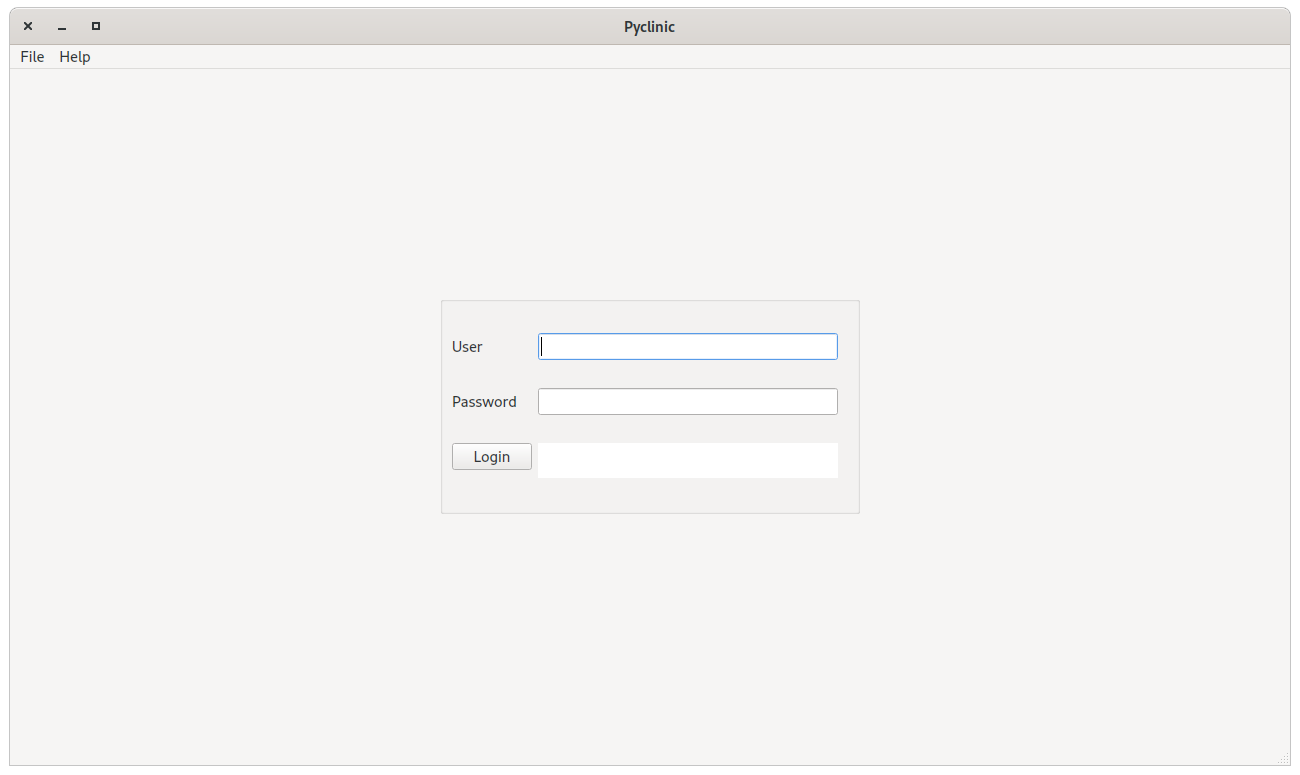
\includegraphics[width=0.8\linewidth]{image/login}
		\caption{\textit{Screenshot} da janela de \textit{login}.}
		\label{fig:PyClinic_login}
	\end{figure}
	
	As ferramentas e/ou funcionalidades ficam separadas sob a forma de abas de modo a que o interface não fique carregado com demasiada informação.
	Por forma a assegurar que dados não são acedidos de forma incorreta, certas funcionalidades do interface ficam bloqueadas até que seja feita uma ação que as liberte como por exemplo escolher um utente antes de entrar no menu de exames.
	
	Ações de uso repetido como aceder a funcionalidades comuns a interfaces ficam mapeadas com atalhos no teclado.
	Funcionalidades críticas como \textit{logout} e sair do programa ficam escondidas numa barra de menu por forma a que o utilizador não as ative por um clique acidental.
	Estes exemplos de design podem ser observados na Figura \ref{fig:PyClinic_edit}.
	
	\begin{figure}[H]
		\centering
		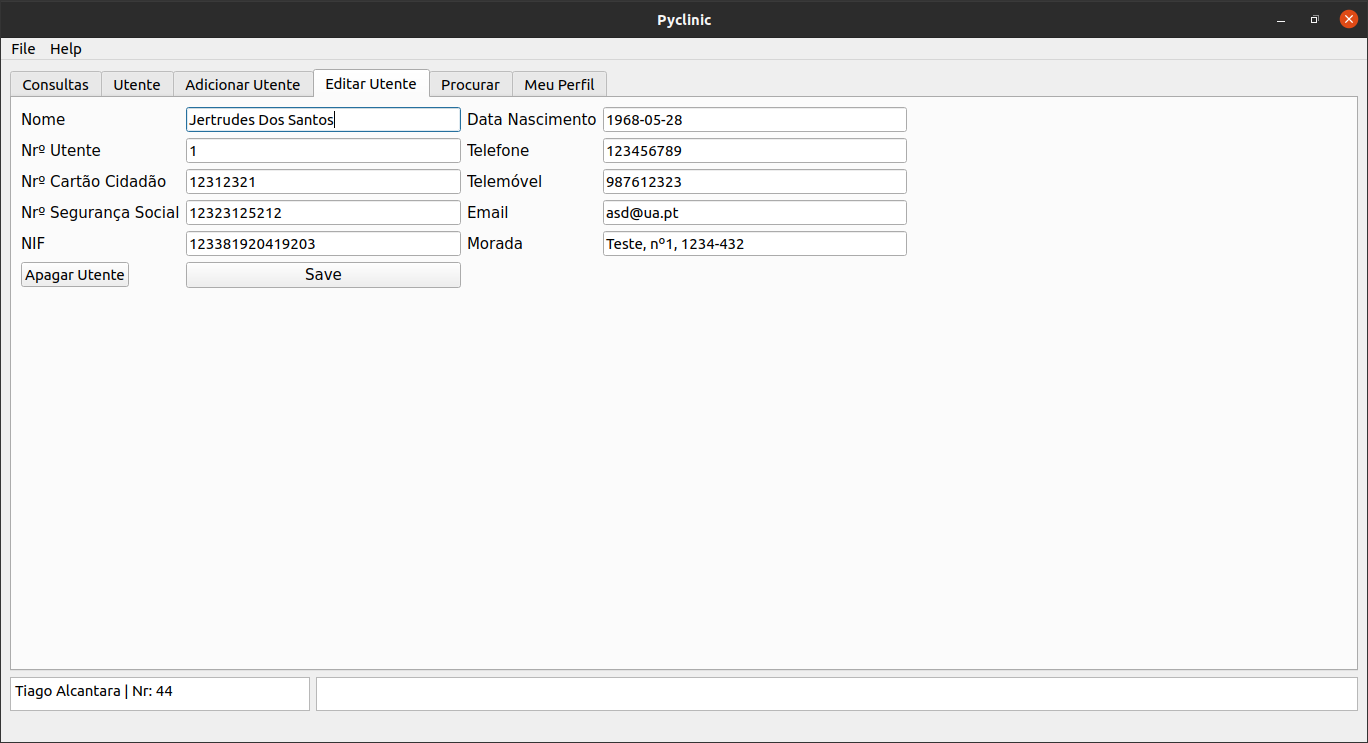
\includegraphics[width=0.8\linewidth]{image/PyClinic_edit}
		\caption{\textit{Screenshot} da janela de rececionista.}
		\label{fig:PyClinic_edit}
	\end{figure}
	
	A navegação entre entradas nos formulários fica simplificada com o uso da tecla "TAB" e garantiu-se que a transição entre entradas é navegada de forma ordeira.
	

\section{Testes de Robustez}
	Nesta fase do projeto, os testes foram realizados ao longo do desenvolvimento da aplicação, nomeadamente na fase final, pois foi nesta fase que o grupo se dedicou mais aos testes para observar o que se podia melhorar e corrigir, para uma melhor apresentação da aplicação.
	
	Os testes realizados consistiam em verificar se a funcionalidade implementada continha o comportamento esperado, e também para verificar a reação da aplicação, caso esta esteja a ser mal utilizada, ou caso o utilizador insira dados incorretos. 
	
	Dependendo dos resultados dos testes, o grupo melhorava algumas funcionalidades, ou corrigia algum erro que aparece-se, para uma melhor interpretação por parte do utilizador.

	 
\chapter{Implementação Base de Dados}

Derivado do modelo de dados persistente, foi elaborado um esquema de SQL, que pode ser verificado na Figura \ref{fig:modelbasedados}, referente aos dados em questão, de forma a que cada elemento da equipa de desenvolvimento fosse capaz de testar o código individualmente, sendo que a \textit{script} foi partilhada pelos elementos do grupo, criando várias bases de dados locais, uma para cada elemento.

Na base de dados surgiu a necessidade identificar que tuplos estão ativos ou inativos, com isto foram definidos atributos adicionais, nomeadamente às relações "id\_funiconário" e "utente",  às quais foi adicionado o atributo "ativo", que define se o funcionário/utente está ativo na clínica. É possível associar este atributo à função de eliminar (quando eliminamos um funcionário, o atributo ativo passa a ser 0 em vez de 1), tal como é possível verificar no modelo físico da base de dados representado pela figura Figura \ref{fig:modelbasedados}.

\begin{figure}[H]
	\centering
	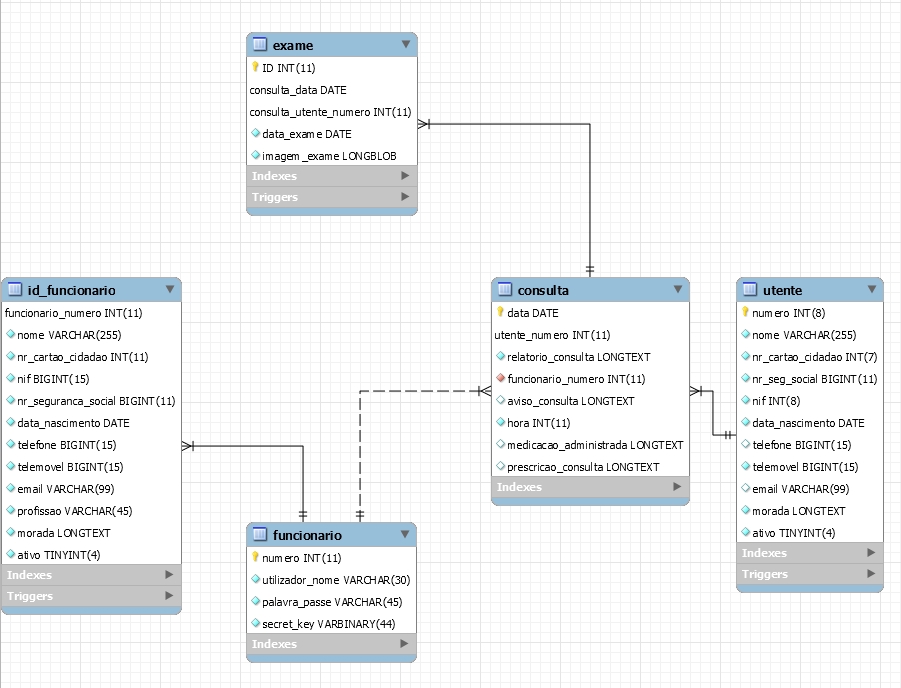
\includegraphics[width=0.8\linewidth]{image/model.png}
	\caption{Modelo físico da Base de Dados SQL.}
	\label{fig:modelbasedados}
\end{figure}

Inicialmente, a base de dados foi elaborada a partir do modelo de classes utilizando engenharia inversa, sendo que foi um método bastante prático para implementar as bases de dados sem qualquer informação prévia, partindo de um modelo desenhado.
Com o evoluir de várias versões da base de dados, esta passou a ficar guardada em ficheiros SQL, de forma a permitir a existência de um utilizador universal presente na primeira utilização (admin) e para simplicidade em termos de implementação do sistema.
Foram também implementados constrangimentos necessários para que o sistema se comporte em conformidade com as restrições previamente mencionadas no Capítulo 2.

Devido à necessidade funcional de colocar a base de dados operacional na rede da Universidade de Aveiro, um esquema atualizado com base neste requisito foi migrado para a base de dados referida atrás.
Aquando da migração das bases de dados locais para a base de dados da rede UA, a utilização de \textit{scripts} (.sql) foi uma mais valia pela fácil atualização dos mesmos para o \textit{schema} e endereço da base de dados, juntamente com a necessidade de deixar um utilizador administrativo pronto para a utilização com a aplicação desenvolvida.

Por fim, tendo um esquema na base de dados online funcional, houve a necessidade de este ser testado exaustivamente até verificada a conformidade com os requisitos estabelecidos.
Na última etapa foram implementados constrangimentos evitando assim que certas verificações se façam em código e que sejam apenas controladas pelo Sistema de Gestão de Bases de Dados.

Funcionalidades como introduzir cliente ou funcionário dependem de \textit{triggers} na base de dados para validar os dados introduzidos, isto permite que outras aplicações a usar a mesma base de dados respeitem as mesmas normas e regras de dados para os respetivos atributos. Embora o objetivo fosse criar \textit{constraints} em vez de \textit{triggers}, a versão do MySQL da base de dados disponibilizada para o projeto (5.7) não suportava a função \textit{"check"}, invalidando a utilização de \textit{constraints} para verificar dados, sendo os \textit{triggers} os substitutos mais corretos.

Atendendo à necessidade de validar valores introduzidos e no que toca aos tipo de valores aceites pela base de dados para cada atributo, foi definido que seriam aplicadas as mesmas normas (já existentes) sobre dados de identificação, obtendo então as seguintes restrições:

\begin{itemize}
	\item Número de segurança social: Contém 11 números e não pode ser nulo.
	\item Número de identificação fiscal: Contém 9 números e não pode ser nulo.
	\item Número de identificação fiscal: Contém 9 números e não pode ser nulo.
	\item Número de identificação civil: Contém 8 números e não pode ser nulo.
	\item Data de nascimento: Segue o formato de AAAA-MM-DD, apenas aceita datas anteriores ao dia em que a mesma está a ser inserida e não pode ser nulo.
	\item Nome: Aceita o nome da pessoa com um máximo de 255 letras e não pode ser nulo.
	\item Telemóvel: Aceita 15 números e não pode ser nulo.
	\item Telefone: Aceita 15 números.
	\item Morada: Aceita uma frase ou texto e não pode ser nulo.
	\item Email: Aceita o email de utilizador com o máximo de 99 letras.
\end{itemize}

\chapter{Conclusões}

Neste projeto foi proposto e implementado com sucesso um \textit{software} de gestão para uma clínica dentária com capacidade para organizar dados e guardar-los numa base de dados possível de ser acedida numa rede interna ou até externa à clínica.

Foi desenvolvido software onde as funcionalidades foram conseguidas com recurso à linguagem de programação Python e o interface gráfico foi desenhado com o programa Qt Designer que usa a \textit{framework} Qt como \textit{backend} para desenhar as janelas.
Para satisfazer a necessidade de guardar/consultar dados de uma forma segura e organizada, foi implementada uma base de dados em linguagem MySQL que fica alojada na rede.
Esta base de dados facilita também a funcionalidade de \textit{login} já que os dados de utilizador ficam também guardados na rede.
Por forma a garantir rastreabilidade de todos os eventos realizados por profissionais de saúde ou de funcionários administrativos, foi implementada uma funcionalidade de \textit{loger} que guarda todos os eventos realizados.
Estima-se que quase todas as funcionalidades propostas foram implementadas com exceção da atualização em tempo real das consultas à base de dados que não foi implementada devido ao grau de complexidade acrescido que não se verificou como justificável durante as últimas etapas do projeto.

Com este projeto o Grupo 5 teve a oportunidade de desenvolver melhor aptidão à linguagem de programação Python, superando assim o seu desafio auto proposto, e também a oportunidade de implementar os conhecimentos adquiridos de bases de dados agora num caso prático virado para um uso real.
Foi também possível ganhar conhecimentos com ferramentas alternativas às que tinham sido propostas para o desenvolvimento de interface, proporcionando-nos assim conhecimentos com o \textit{software} estado de arte usado pelas principais empresas de desenvolvimento de aplicações gráficas.

Olhando para o futuro, conseguimos imaginar melhorias que podem ser implementadas, como por exemplo no desenvolvimento da interface usar botões ou descrições que usem ficheiros com tabelas de nome/descrição por forma a que seja possível distribuir o \textit{software} com capacidade de trocar de língua, trocando apenas no código um ficheiro que contém todo o texto a ser desenhado para a língua em questão.
De um ponto de vista funcional seria também interessante implementar funcionalidades para alertar um utente, por email ou telefone, de uma consulta quando esta se estiver a aproximar.

\bibliographystyle{ieeetr}
\bibliography{ref}

\end{document}          
